% Báo cáo đồ án Project 3 theo mẫu IEEE Conference của phần seminar
% (vkgqa/ieee_template/conference_101719.tex).
% Biên dịch: latexmk -xelatex project3_ieee.tex  (hoặc xelatex 2 lần)
\documentclass[conference]{IEEEtran}
\IEEEoverridecommandlockouts
\usepackage{fontspec}
\setmainfont{Times New Roman}
\usepackage[vietnamese]{babel}
\usepackage{cite}
\usepackage{amsmath,amssymb,amsfonts}
\usepackage{icomma}
\usepackage{graphicx}
\usepackage{textcomp}
\usepackage{xcolor}
\usepackage{booktabs}
\usepackage{multirow}
\usepackage{array}
\usepackage{tikz}
\usetikzlibrary{arrows.meta,positioning}
\usepackage{pgfplots}
\pgfplotsset{compat=1.17}
\usepackage[hidelinks]{hyperref}
\usepackage{url}

\makeatletter
\newcommand{\linebreakand}{\end{@IEEEauthorhalign}\hfill\mbox{}\par\mbox{}\hfill\begin{@IEEEauthorhalign}}
\makeatother

\newcommand{\code}[1]{\texttt{#1}}
\newcommand{\mrr}{MRR@100}
\newcommand{\pmm}{$\pm$}
\newcommand{\GHrepo}{https://github.com/FluteInTheRain/graph-semantic-image-editing}

\renewcommand{\IEEEkeywordsname}{Từ khóa}
\addto\captionsvietnamese{\renewcommand{\refname}{Tài liệu tham khảo}\renewcommand{\abstractname}{Tóm tắt}\renewcommand{\tablename}{Bảng}\renewcommand{\figurename}{Hình}}

\begin{document}

% Trang bìa riêng, một cột (cùng kiểu báo cáo seminar)
\begin{titlepage}
\onecolumn
\centering
{\large ĐẠI HỌC QUỐC GIA THÀNH PHỐ HỒ CHÍ MINH\par}
{\large\bfseries TRƯỜNG ĐẠI HỌC KHOA HỌC TỰ NHIÊN\par}
\vspace{4mm}
\rule{0.6\textwidth}{0.6pt}\par
\vspace{30mm}
{\Large\bfseries BÁO CÁO ĐỒ ÁN\par}
\vspace{4mm}
{\large Môn học: MTH084 -- Học máy trên dữ liệu đồ thị\par}
\vspace{18mm}
{\LARGE\bfseries Truy vấn ảnh bằng văn bản có đồ thị\\[2mm]
và giải thích trung thực\par}
\vspace{10mm}
\begin{minipage}{0.82\textwidth}
\centering\large
Project 3: Multimodal Retrieval và xAI trên đồ thị tri thức đa phương thức
\end{minipage}
\vfill
\begin{tabular}{ll}
\textbf{Học viên thực hiện:} & … -- … \\
                              & Nguyễn Thiện Thuật -- 25C15025 \\
                              & Nguyễn Phước Thiện -- 25C15060 \\
                              & Quan Phú Long -- 25C15050 \\
                              & Trần Hồ Thanh Vũ -- 25C15068 \\[2mm]
\textbf{Giảng viên hướng dẫn:} & … \\
\end{tabular}
\vspace{20mm}

{\large Thành phố Hồ Chí Minh, tháng 11 năm 2026\par}
\end{titlepage}
\twocolumn
\setcounter{page}{1}


\title{Đồ thị có thật sự giúp truy vấn ảnh bằng văn bản? Xếp hạng lại CLIP bằng GraphSAGE, giải thích trung thực và chuyển giao sang MMKG tiếng Việt}

\author{
\IEEEauthorblockN{…}
\IEEEauthorblockA{MSHV: …}
\and
\IEEEauthorblockN{Nguyễn Thiện Thuật}
\IEEEauthorblockA{MSHV: 25C15025}
\and
\IEEEauthorblockN{Nguyễn Phước Thiện}
\IEEEauthorblockA{MSHV: 25C15060}
\linebreakand
\IEEEauthorblockN{Quan Phú Long}
\IEEEauthorblockA{MSHV: 25C15050}
\and
\IEEEauthorblockN{Trần Hồ Thanh Vũ}
\IEEEauthorblockA{MSHV: 25C15068}
\linebreakand
\IEEEauthorblockA{\textit{Trường Đại học Khoa học Tự nhiên, ĐHQG TP.HCM}}
}

\maketitle

\begin{abstract}
Truy vấn ảnh bằng CLIP chỉ so cosine giữa vectơ của câu và vectơ của ảnh, nên hệ thống không dùng đến quan hệ giữa các khái niệm có trong ảnh và cũng không cho biết vì sao một ảnh được trả về. Báo cáo này trình bày một hệ thống gồm ba bước. CLIP ViT-B/32 được giữ đóng băng để lấy 100 ảnh ứng viên. Tiếp theo, một đồ thị hai phía ảnh-khái niệm (3.880 synset WordNet) và một lớp GraphSAGE được dùng để xếp hạng lại các ứng viên này. Mỗi kết quả được giải thích bằng các cạnh ảnh-khái niệm, tính bằng can thiệp trên chính mô hình xếp hạng. Trên tập test Visual Genome (5.000 ảnh, 25.000 truy vấn, 3 seed), \mrr{} tăng từ 0,1076 lên 0,1284. Tuy vậy, mô hình đối chứng không dùng đồ thị đã đạt 0,1266 và mô hình trên đồ thị xáo cạnh đạt 0,1272. Khoảng 91\% mức tăng đến từ phép chiếu tuyến tính học được; phần đóng góp của đồ thị nhỏ nhưng ổn định qua các seed và thể hiện rõ nhất ở các truy vấn chung chung. Kết luận ``phần lớn mức tăng đến từ phép chiếu'' lặp lại trên tập thứ hai Flickr30k và với phần truy xuất đồ thị con của G-Retriever (2024); trên hai thí nghiệm này, đồ thị không tốt hơn mô hình không đồ thị. Giải thích bằng Integrated Gradients trung thực với mô hình: trên test, bỏ 10 cạnh giải thích làm ảnh tụt trung bình 2,57 bậc, trong khi bỏ 10 cạnh ngẫu nhiên chỉ làm tụt 0,26 bậc ($p = 0{,}0005$). Nhóm cũng tự xây một đồ thị tri thức đa phương thức tiếng Việt về di tích và di sản (119 thực thể, 303 bộ ba, 380 ảnh). Mô hình học trên Visual Genome chuyển sang miền này mà không cần huấn luyện lại, nhưng truy vấn tiếng Việt thất bại do bộ mã hóa văn bản của CLIP.
\end{abstract}

\begin{IEEEkeywords}
truy vấn đa phương thức, CLIP, GraphSAGE, xếp hạng lại, G-Retriever, AI có thể giải thích, fidelity, đồ thị tri thức đa phương thức
\end{IEEEkeywords}

\section{Giới thiệu}
\label{sec:intro}
Bài toán truy vấn ảnh bằng văn bản (text-to-image retrieval) nhận một câu như ``a girl wearing blue jeans'' và trả về danh sách ảnh xếp theo mức độ phù hợp. Cách làm phổ biến hiện nay là mã hóa câu và ảnh vào cùng một không gian bằng CLIP~\cite{radford2021clip} rồi xếp ảnh theo cosine. Cách này cho kết quả tốt nhưng có hai hạn chế. Thứ nhất, CLIP không khai thác quan hệ có cấu trúc giữa các thực thể và khái niệm. Thứ hai, điểm cosine không giải thích được vì sao một ảnh được xếp lên đầu.

Đề bài yêu cầu đưa dữ liệu đồ thị vào bài toán này: dùng đồ thị để cải thiện thứ hạng, sau đó giải thích mỗi kết quả bằng chính các quan hệ hoặc đồ thị con đã tham gia vào việc xếp hạng. Vì vậy đồ án tập trung đo phần đóng góp của đồ thị và không xây mô hình thị giác mới. Nhóm đặt ra ba câu hỏi nghiên cứu, tương ứng với ba nhiệm vụ của đề bài:
\begin{itemize}
\item \textbf{RQ1} (truy vấn): trên một giao thức đánh giá chuẩn, CLIP thuần và CLIP kết hợp đồ thị đạt kết quả đến đâu?
\item \textbf{RQ2} (vai trò của đồ thị): phần cải thiện có thật sự đến từ cấu trúc quan hệ không, và đồ thị giúp ở nhóm truy vấn nào?
\item \textbf{RQ3} (giải thích): những cạnh nào đã đẩy một ảnh lên, và giải thích đó có trung thực với cơ chế xếp hạng hay không?
\end{itemize}

Nhóm chọn nhánh văn bản $\to$ ảnh trên Visual Genome~\cite{krishna2017vg}, đo thêm chiều ảnh $\to$ văn bản như một phép đo mở rộng. Các đóng góp chính của đồ án gồm:
\begin{enumerate}
\item Một cách chia dữ liệu cố định cho Visual Genome có gom các ảnh gần trùng, kèm một giao thức đánh giá coi mọi ảnh có cùng câu mô tả là đáp án đúng (Mục~\ref{sec:data}).
\item Một mô hình GraphSAGE một lớp được khởi tạo sao cho ban đầu cho kết quả đúng bằng CLIP, sau đó được huấn luyện trực tiếp cho việc xếp hạng lại; kèm theo là bộ mô hình đối chứng để tách riêng phần đóng góp của đồ thị (Mục~\ref{sec:method} và~\ref{sec:retrieval}).
\item Kết quả chạy lại toàn bộ pipeline trên tập công khai thứ hai Flickr30k và kết quả tái lập phần truy xuất đồ thị con của G-Retriever~\cite{he2024gretriever}, một phương pháp công bố năm 2024.
\item Một quy trình giải thích tính bằng can thiệp trên chính mô hình, có bước kiểm tra rằng mô hình được giải thích đúng là mô hình đã báo cáo, và được đánh giá bằng fidelity, validity, sparsity so với đối chứng ngẫu nhiên (Mục~\ref{sec:xai}).
\item Một đồ thị tri thức đa phương thức (MMKG) tiếng Việt do nhóm tự xây, dùng để đo khả năng chuyển miền, chuyển ngôn ngữ của mô hình và của giải thích (Mục~\ref{sec:mmkg}).
\end{enumerate}

Bảng~\ref{tab:status} tóm tắt mức độ hoàn thành theo các cấp độ của đề. Toàn bộ mã nguồn, cấu hình, quyết định thiết kế (ADR) và bảng số nằm trong kho mã của nhóm\footnote{\url{\GHrepo}}. Các kết quả chính được chép từ \code{results/tables/*.csv}; một số đại lượng dẫn xuất (tỉ lệ, hiệu ghép cặp) được tính từ các bảng này, số còn lại lấy từ hồ sơ thí nghiệm và ADR trong kho mã.

\begin{table}[t]
\centering
\caption{Mức độ hoàn thành theo các cấp độ của đề bài}
\label{tab:status}
\footnotesize
\setlength{\tabcolsep}{3pt}
\begin{tabular}{@{}>{\raggedright\arraybackslash}p{1.15cm}>{\raggedright\arraybackslash}p{4.35cm}>{\raggedright\arraybackslash}p{2.1cm}@{}}
\toprule
\textbf{Cấp độ} & \textbf{Yêu cầu} & \textbf{Tình trạng} \\
\midrule
1 & CLIP, đồ thị, GNN, xếp hạng lại, 3 seed, ablation, phân tích 5+5 truy vấn & Hoàn thành \\
1 mở rộng & nDCG@10, chiều ảnh $\to$ văn bản, nhóm truy vấn & Hoàn thành \\
2 & Tập công khai thứ hai (Flickr30k) & Hoàn thành \\
2 & Phương pháp từ năm 2024 (G-Retriever) & Hoàn thành, kết quả âm \\
2 & Bộ $\ge$20 truy vấn trực tiếp/gián tiếp & Hoàn thành: 38 câu trên VG (CLIP thuần, đối chứng, G-Retriever); 318 câu trên MMKG \\
3 & Fidelity, validity, sparsity trên $\ge$10 truy vấn & Hoàn thành \\
3 & MMKG tiếng Việt tự xây & Hoàn thành \\
4 & Cải tiến riêng của nhóm & Chưa làm \\
Sản phẩm & Giao diện demo, slide & Hoàn thành \\
\bottomrule
\end{tabular}
\end{table}

\section{Cơ sở lý thuyết và công trình liên quan}
\label{sec:background}

\subsection{Truy vấn văn bản--ảnh bằng CLIP}
CLIP~\cite{radford2021clip} huấn luyện song song một bộ mã hóa ảnh $f_I$ và một bộ mã hóa văn bản $f_T$ bằng học tương phản trên các cặp ảnh--chú thích. Sau khi chuẩn hóa L2, độ phù hợp giữa truy vấn $q$ và ảnh $i$ là $\cos(f_T(q), f_I(i))$, và việc tìm kiếm quy về tìm láng giềng gần nhất. Nhóm dùng bản OpenCLIP~\cite{cherti2023openclip} ViT-B/32 huấn luyện trên LAION-2B~\cite{schuhmann2022laion}, giữ đóng băng toàn bộ, và dùng FAISS~\cite{johnson2019faiss} với chỉ mục \code{IndexFlatIP} để tìm kiếm chính xác.

\subsection{Mạng nơ-ron đồ thị}
Mạng nơ-ron đồ thị (GNN) cập nhật biểu diễn của một đỉnh bằng cách gom thông tin từ các đỉnh láng giềng. GCN~\cite{kipf2017gcn} lấy trung bình có chuẩn hóa theo bậc, GAT~\cite{velickovic2018gat} dùng trọng số chú ý, còn GraphSAGE~\cite{hamilton2017sage} tách riêng phần của chính đỉnh và phần của láng giềng:
\begin{equation}
h_v = W_{\text{self}}\,x_v + W_{\text{nb}}\cdot \operatorname{mean}_{u\in N(v)} x_u + b.
\end{equation}
Nhóm chọn GraphSAGE vì cách tách này cho phép khởi tạo mô hình bằng đúng CLIP và giúp việc giải thích đơn giản hơn (Mục~\ref{sec:model}). Phần cài đặt dùng \code{SAGEConv} của PyTorch Geometric~\cite{fey2019pyg}.

\subsection{Đồ thị tri thức đa phương thức}
Scene graph của Visual Genome~\cite{krishna2017vg} mô tả đối tượng, thuộc tính và quan hệ trong từng ảnh. Đồ thị tri thức đa phương thức (multimodal knowledge graph, MMKG) gắn ảnh vào các thực thể của một đồ thị tri thức; khảo sát của Chen và cộng sự~\cite{chen2024kgmm} tổng hợp các hướng nghiên cứu chính. Những phương pháp MMKG gần đây được đề bài gợi ý, như MKGformer~\cite{chen2022mkgformer}, NativE~\cite{zhang2024native} và AdaMF-MAT~\cite{zhang2024adamf}, giải bài toán hoàn thiện đồ thị (dự đoán liên kết) trên các bộ MKG-W, MKG-Y hay FB15k-237-IMG. Chúng không áp dụng trực tiếp được cho bài toán xếp hạng ảnh theo câu truy vấn của nhóm.

Gần với bài toán của nhóm hơn là G-Retriever~\cite{he2024gretriever}, một phương pháp hỏi đáp trên đồ thị có thuộc tính văn bản. G-Retriever chấm độ liên quan của từng đỉnh với câu hỏi, chọn một đồ thị con liên thông bằng bài toán cây Steiner có thưởng (prize-collecting Steiner tree, PCST)~\cite{hegde2015pcst}, mã hóa đồ thị con bằng GNN rồi đưa cho mô hình ngôn ngữ lớn sinh câu trả lời. Bước chọn đồ thị con phụ thuộc vào câu hỏi, và đó là phần nhóm tái lập trong Mục~\ref{sec:gret}.

\subsection{Giải thích GNN và đánh giá giải thích}
Ba nhóm phương pháp giải thích được dùng trong đồ án:
\begin{itemize}
\item \textbf{Occlusion}: xóa lần lượt từng cạnh và đo điểm thay đổi bao nhiêu. Cách này đơn giản và bám sát mô hình, nhưng cần một lần chạy cho mỗi cạnh.
\item \textbf{Integrated Gradients} (IG)~\cite{sundararajan2017ig}: gán cho mỗi cạnh một trọng số rồi tích phân gradient của điểm theo trọng số đó từ 0 đến 1.
\item \textbf{GNNExplainer}~\cite{ying2019gnnexplainer}: học một mặt nạ cạnh vừa giữ được dự đoán vừa thưa nhất có thể.
\end{itemize}
Để đánh giá, GraphFramEx~\cite{amara2022graphframex} tách Fid$^+$ (bỏ phần giải thích thì dự đoán thay đổi bao nhiêu, phản ánh tính cần thiết) và Fid$^-$ (chỉ giữ phần giải thích thì dự đoán thay đổi bao nhiêu, phản ánh tính đủ), rồi gộp hai đại lượng thành chỉ số characterization. Zheng và cộng sự~\cite{zheng2024robust} chỉ ra rằng xóa cạnh tạo ra những đồ thị lệch khỏi phân phối lúc huấn luyện, và đề xuất robust fidelity, trong đó mỗi cạnh chỉ bị xóa với một xác suất nhất định.

Yêu cầu xuyên suốt của đề là giải thích phải xuất phát từ chính cơ chế xếp hạng. Một đường đi ``hợp lý'' được tìm sau khi đã có kết quả, nếu không ảnh hưởng tới dự đoán, thì không được coi là giải thích. Vì vậy nhóm chỉ dùng các phương pháp chạy lại đúng mô hình xếp hạng trên đồ thị đã bị sửa.

\section{Dữ liệu và chống rò rỉ}
\label{sec:data}

\subsection{Visual Genome}
Visual Genome v1.2~\cite{krishna2017vg} (giấy phép CC BY 4.0) có 108.077 ảnh và 5.408.689 câu mô tả vùng (region description). Với mỗi ảnh, nhóm lấy mẫu 5 câu mô tả vùng (riêng một ảnh chỉ có 3 câu), tổng cộng 540.383 câu. Ảnh và câu được mã hóa một lần bằng OpenCLIP ViT-B/32 (\code{laion2b\_s34b\_b79k}) trên Kaggle, lưu dưới dạng \code{.npz} để cả nhóm dùng chung. Phần dựng đồ thị dùng thêm tệp \code{objects.json} v1.4 với 2.516.939 đối tượng, trong đó 19,6\% không gắn được synset WordNet~\cite{miller1995wordnet} và 1.793 ảnh không có đối tượng nào. Thông tin nguồn, giấy phép và mã sha256 của từng tệp được ghi trong data card \code{data\_cards/visual\_genome.md}.

\subsection{Chia tập cố định và xử lý ảnh trùng}
Visual Genome không có cách chia chính thức. Nhóm chia theo \emph{ảnh}: 5.000 ảnh test, 5.000 ảnh val và 98.077 ảnh train; mỗi câu thuộc về tập của ảnh tương ứng. Dữ liệu có ảnh trùng: 5 cặp ảnh có embedding giống hệt nhau và 247 cặp có cosine $\ge 0,99$ (ví dụ ảnh \code{285982} và \code{2375578} có cosine 0,99992). Nếu hai bản của cùng một ảnh rơi vào train và test, dữ liệu sẽ bị rò rỉ. Vì vậy các ảnh có cosine $\ge 0,99$ được gom thành nhóm theo quan hệ bắc cầu (A gần trùng B, B gần trùng C thì cả ba chung nhóm) và cả nhóm luôn nằm trong cùng một tập. Ngưỡng này được chốt trước khi có bất kỳ kết quả truy vấn nào. Tệp chia tập \code{split\_seed0.json} được commit cùng mã sha256 và là nguồn duy nhất cho mọi thí nghiệm; chạy lại script cho ra tệp giống hệt từng byte.

\subsection{Giao thức đánh giá}
\label{sec:protocol}
Truy vấn là toàn bộ câu mô tả vùng đã lấy mẫu của ảnh test (25.000 câu), kho tìm kiếm là 5.000 ảnh test. Một ảnh được coi là đáp án đúng nếu nó có một câu trùng với truy vấn (cosine văn bản $\ge 0,9999$, ngưỡng này chỉ để bù sai số số học), kể cả ảnh gốc của câu. Lý do là 26\% số câu trong dữ liệu bị trùng, ví dụ ``a man'' hay ``white clouds''; nếu chỉ tính ảnh gốc là đúng thì CLIP bị đánh giá thấp một cách sai lệch. Trên tập test, 11,28\% truy vấn có nhiều hơn một đáp án.

Các chỉ số dùng trong báo cáo là Recall@1/5/10, \mrr{} (ảnh đúng nằm ngoài 100 kết quả đầu được tính bằng 0) và nDCG@10 nhị phân~\cite{jarvelin2002ndcg}. Vì mỗi ảnh chỉ xét 5 câu, Recall tuyệt đối là một cận dưới; so sánh giữa các mô hình vẫn công bằng vì mọi mô hình dùng chung định nghĩa. CLIP thuần và CLIP kết hợp đồ thị gọi cùng một hàm lấy 100 ứng viên, nên hai mô hình chỉ khác nhau ở thứ tự sắp xếp bên trong 100 ảnh đó.

\subsection{Các quy tắc chống rò rỉ}
Nhóm áp dụng năm quy tắc, đều được ghi thành ADR trước khi chạy thí nghiệm:
\begin{enumerate}
\item Từ vựng khái niệm, từ điển tên đối tượng $\to$ synset và cạnh đồng xuất hiện chỉ được đếm trên tập train. Một bài kiểm thử tự động xác nhận rằng ảnh test không làm thay đổi từ vựng.
\item Cạnh của ảnh val và test chỉ phụ thuộc vào vectơ CLIP của chính ảnh đó, không dùng nhãn (Mục~\ref{sec:graph}).
\item Mọi lựa chọn (learning rate, epoch, $\alpha$, phương pháp giải thích, số cạnh $m$) đều làm trên val. Tập test được chạy đúng một lần cho mỗi seed; script từ chối lần chạy thứ hai của cùng một thí nghiệm và seed.
\item Quy tắc chọn cấu hình chính và quy tắc của các ablation được commit trước khi chạy test. Kết quả âm vẫn được báo cáo.
\item Seed 0, 1, 2 chỉ thay đổi phần huấn luyện (thứ tự batch, mẫu âm khó); cách chia tập giữ nguyên. Vì CLIP được đóng băng và FAISS Flat là tất định, kết quả của CLIP thuần có độ lệch chuẩn bằng 0.
\end{enumerate}

\subsection{Flickr30k}
Tập công khai thứ hai là Flickr30k~\cite{young2014flickr} theo bản phân chia của Karpathy~\cite{karpathy2015}, gồm 31.014 ảnh, mỗi ảnh có 5 chú thích. Embedding được trích bằng cùng mô hình CLIP như Visual Genome. Nhóm chia lại tập theo đúng quy trình trên (21.014 ảnh train, 5.000 val, 5.000 test, seed 0; có 2 cặp ảnh cosine $\ge 0,99$ được gom chung) và không dùng trường \code{split} có sẵn của bản Karpathy. Truy vấn là cả 5 chú thích của mỗi ảnh val/test (25.000 câu); chỉ 0,08\% truy vấn val có hơn một đáp án.

Flickr30k không có annotation đối tượng nên không đếm được từ vựng khái niệm như trên Visual Genome. Nhóm chép nguyên 3.880 đỉnh khái niệm (synset và vectơ văn bản CLIP) từ đồ thị Visual Genome, rồi nối mỗi ảnh Flickr30k với 16 khái niệm gần nhất theo cosine CLIP, được tổng cộng 496.224 cạnh. Vì từ vựng chỉ được đếm trên train Visual Genome và cạnh của mỗi ảnh chỉ phụ thuộc vào vectơ của chính ảnh đó, quy trình này không làm rò rỉ thông tin từ test Flickr30k. Mô hình có cạnh đồng xuất hiện (cần annotation đối tượng) và phần phân nhóm truy vấn (luật được chốt trên câu Visual Genome) không được chạy trên Flickr30k.

\subsection{MMKG tiếng Việt tự xây}
\label{sec:mmkg-data}
Nhóm chọn miền hẹp là \emph{di tích và di sản Việt Nam}: các thực thể có danh hiệu di sản trên Wikidata (\code{P1435}) và thuộc Việt Nam (\code{P17 = Q881}). Thực thể, bộ ba và ảnh được thu tự động từ Wikidata và Wikimedia Commons. Dữ liệu thô (snapshot) được lưu nguyên trạng rồi mới lọc ở bước dựng, nên mọi bước lọc đều kiểm tra lại được. Quy trình gồm ba bước:
\begin{enumerate}
\item \textbf{Thu thập}: lấy mọi phát biểu của thực thể trong miền trỏ tới một thực thể Wikidata khác. Dữ liệu thô có 848 thực thể, 3.581 bộ ba và 5.093 cặp (thực thể, ảnh) ứng viên.
\item \textbf{Dựng}: chỉ giữ 18 thuộc tính Wikidata, đổi thành 17 quan hệ như \code{heritage\_designation}, \code{instance\_of}, \code{kept\_at}, \code{made\_from}, \code{located\_in}, \code{culture}. Ảnh phải là \code{P18} của thực thể hoặc nằm trực tiếp trong danh mục Commons của nó; ảnh thuộc nhiều thực thể, ảnh không phải dạng raster, ảnh có cạnh ngắn dưới 224 px và ảnh có giấy phép không mở đều bị loại. Mỗi hiện vật giữ từ 3 đến 5 ảnh.
\item \textbf{Duyệt}: toàn bộ 962 dòng được một mô hình AI duyệt sơ bộ, sau đó một thành viên duyệt lại từng dòng. Ảnh có mặt người, ảnh không đúng hiện vật và ảnh trùng bị loại.
\end{enumerate}
Bộ chính thức có 119 thực thể (80 hiện vật có ảnh và 39 khái niệm, tất cả đều có tên tiếng Việt), 303 bộ ba và 380 ảnh. Mọi ảnh có giấy phép tự do (CC0, public domain, CC BY, CC BY-SA), kèm tác giả và đường dẫn nguồn. Các quan hệ nhiều nhất là \code{heritage\_designation} (86), \code{instance\_of} (65), \code{kept\_at} (45) và \code{made\_from} (30). Thông tin đầy đủ về nguồn, giấy phép, cách tạo bộ ba và hạn chế của dữ liệu nằm trong \code{data\_cards/mmkg\_vi.md}.

\begin{figure}[t]
\centering
\begin{tikzpicture}[
  ent/.style={draw=blue!60!black,thick,rounded corners=2pt,fill=blue!6,font=\scriptsize,align=center,text width=2.0cm,minimum height=0.6cm},
  con/.style={draw=orange!70!black,rounded corners=6pt,fill=orange!8,font=\scriptsize,align=center,text width=1.9cm,minimum height=0.5cm},
  pic/.style={draw=gray,fill=gray!10,font=\tiny,minimum width=0.6cm,minimum height=0.45cm},
  r/.style={-{Stealth[length=1.4mm]},thick,blue!50!black},
  lab/.style={font=\tiny,fill=white,inner sep=1pt}]
\node[ent] (h) at (0,0) {Hiện vật\\(\code{item})};
\node[con] (t1) at (-2.4,1.5) {Bảo vật quốc gia};
\node[con] (t2) at (2.4,1.5) {Văn hóa Đông Sơn};
\node[con] (t3) at (-2.4,-1.4) {Đồng thanh};
\node[con] (t4) at (2.4,-1.4) {Bảo tàng};
\draw[r] (h) -- node[lab]{\code{heritage\_designation}} (t1);
\draw[r] (h) -- node[lab]{\code{culture}} (t2);
\draw[r] (h) -- node[lab]{\code{made\_from}} (t3);
\draw[r] (h) -- node[lab]{\code{kept\_at}} (t4);
\node[pic] (p1) at (-0.75,-2.3) {ảnh};
\node[pic] (p2) at (0,-2.3) {ảnh};
\node[pic] (p3) at (0.75,-2.3) {ảnh};
\draw[gray,thick] (h) -- (p1); \draw[gray,thick] (h) -- (p2); \draw[gray,thick] (h) -- (p3);
\end{tikzpicture}
\caption{Lược đồ MMKG tiếng Việt: mỗi hiện vật nối với các khái niệm qua 17 loại quan hệ lấy từ Wikidata và có 3--5 ảnh từ Wikimedia Commons. Câu truy vấn gián tiếp được sinh từ các bộ ba này.}
\label{fig:mmkg}
\end{figure}

Hình~\ref{fig:mmkg} mô tả lược đồ của MMKG. Từ MMKG, nhóm sinh tự động 318 truy vấn. Mỗi hiện vật có một câu \emph{trực tiếp} gọi tên hiện vật và một câu \emph{gián tiếp} giấu tên, chỉ mô tả hiện vật qua các bộ ba của nó (ví dụ ``a heritage of Vietnam, made of bronze, of the Dong Son culture, kept at National Museum of Vietnamese History''). Mỗi câu có một bản tiếng Anh và một bản tiếng Việt cùng nội dung. Đáp án là mọi ảnh của mọi hiện vật khớp với câu. Câu gián tiếp được chia thành loại \emph{cụ thể} (chỉ một hiện vật khớp, 35 câu mỗi ngôn ngữ) và loại \emph{chung chung} (nhiều hiện vật khớp, 44 câu). Một hiện vật không có bộ ba nào nên không có câu gián tiếp. MMKG chỉ được dùng để đánh giá; không có lựa chọn nào được thực hiện trên bộ này.

\section{Phương pháp}
\label{sec:method}

\subsection{Pipeline tổng thể}
Hình~\ref{fig:pipeline} mô tả pipeline theo quy trình đề bài gợi ý: truy vấn đi qua CLIP, lấy top-100 ảnh theo cosine, tính điểm đồ thị cho từng ứng viên, xếp hạng lại, sinh giải thích và cuối cùng đo độ trung thực của giải thích.

\begin{figure}[t]
\centering
\begin{tikzpicture}[
  node distance=0.32cm and 0.3cm,
  box/.style={draw=blue!60!black,thick,rounded corners=2pt,fill=blue!5,align=center,font=\scriptsize,minimum height=0.85cm,text width=1.45cm},
  data/.style={draw=gray,dashed,rounded corners=2pt,fill=gray!5,align=center,font=\scriptsize,text width=1.45cm,minimum height=0.7cm},
  arr/.style={-{Stealth[length=1.6mm]},thick,blue!50!black}]
\node[data] (q) {Truy vấn $q$};
\node[box,right=of q] (clip) {CLIP $f_T$\\(đóng băng)};
\node[box,right=of clip] (faiss) {FAISS\\top-100};
\node[box,right=of faiss] (gnn) {GraphSAGE\\điểm $g$};
\node[box,below=0.6cm of gnn] (fuse) {Kết hợp\\{\tiny $\alpha\cos+(1{-}\alpha)g$}};
\node[box,left=of fuse] (exp) {Giải thích\\cạnh $i$--$c$};
\node[box,left=of exp] (fid) {Fidelity,\\validity};
\node[data,above=0.45cm of faiss] (img) {Ảnh $f_I$\\(tính trước)};
\node[data,above=0.45cm of gnn] (graph) {Đồ thị\\ảnh--khái niệm};
\draw[arr] (q) -- (clip); \draw[arr] (clip) -- (faiss); \draw[arr] (faiss) -- (gnn);
\draw[arr] (img) -- (faiss); \draw[arr] (graph) -- (gnn);
\draw[arr] (gnn) -- (fuse); \draw[arr] (fuse) -- (exp); \draw[arr] (exp) -- (fid);
\end{tikzpicture}
\caption{Pipeline của hệ thống. Ô nét đứt là dữ liệu được tính trước một lần.}
\label{fig:pipeline}
\end{figure}

\subsection{Đồ thị ảnh--khái niệm}
\label{sec:graph}
Đồ thị có hai loại đỉnh. Đỉnh ảnh gồm mọi ảnh trong tập, kể cả ảnh không có đối tượng nào. Đỉnh khái niệm gồm 3.880 synset WordNet xuất hiện trong ít nhất 5 ảnh train. Vectơ của ảnh là embedding CLIP; vectơ của khái niệm là embedding văn bản CLIP của câu ``a photo of a \{lemma\}'' (ví dụ \code{fire\_hydrant.n.01} trở thành ``a photo of a fire hydrant''). Nhờ vậy ảnh và khái niệm nằm trong cùng một không gian 512 chiều.

\textbf{Cạnh \code{contains} (khái niệm $\to$ ảnh).} Phiên bản đầu tiên lấy cạnh từ annotation đối tượng và gặp hai vấn đề. Nếu ảnh test dùng annotation, hệ thống đọc được thông tin mà một ảnh mới ngoài thực tế không có. Còn nếu chỉ tập train dùng annotation, tập test thì không, hai phân phối sẽ khác nhau. Vì vậy phiên bản chính nối mỗi ảnh với $k = 16$ khái niệm có cosine CLIP cao nhất, áp dụng như nhau cho train, val và test. Giá trị $k = 16$ gần với bậc trung bình của đồ thị annotation (1.719.645 cạnh trên 108.077 ảnh, xấp xỉ 15,9). Đồ thị có 1.569.232 cạnh ở train và 80.000 cạnh ở mỗi tập val, test.

\begin{figure}[t]
\centering
\begin{tikzpicture}[
  img/.style={draw=blue!60!black,thick,rounded corners=2pt,fill=blue!6,font=\scriptsize,align=center,minimum width=1.5cm,minimum height=0.7cm},
  con/.style={draw=orange!70!black,rounded corners=6pt,fill=orange!8,font=\scriptsize,minimum height=0.45cm,inner sep=2pt},
  e/.style={-{Stealth[length=1.4mm]},blue!50!black},
  co/.style={dashed,red!60!black}]
\node[img] (i1) at (0,0) {Ảnh $i_1$\\(train)};
\node[img] (i2) at (5.4,0) {Ảnh $i_2$\\(test)};
\node[con] (c1) at (1.2,1.7) {\code{horse.n.01}};
\node[con] (c2) at (2.7,2.4) {\code{saddle.n.01}};
\node[con] (c3) at (4.2,1.7) {\code{rein.n.01}};
\node[con] (c4) at (2.7,0.9) {\code{man.n.01}};
\node[con] (c5) at (2.7,-1.1) {\code{beach.n.01}};
\draw[e] (c1) -- (i1); \draw[e] (c2) -- (i1); \draw[e] (c4) -- (i1); \draw[e] (c5) -- (i1);
\draw[e] (c1) -- (i2); \draw[e] (c3) -- (i2); \draw[e] (c4) -- (i2);
\draw[co] (c1) -- (c2); \draw[co] (c2) -- (c3); \draw[co] (c1) -- (c3);
\node[font=\tiny,align=left,anchor=west] at (-0.6,-1.75) {\tikz\draw[-{Stealth[length=1.4mm]},blue!50!black](0,0)--(0.4,0); \code{contains}: 16 khái niệm gần nhất theo CLIP \quad \tikz\draw[dashed,red!60!black](0,0)--(0.4,0); \code{cooccurs\_with}: PMI trên train};
\end{tikzpicture}
\caption{Minh họa đồ thị ảnh--khái niệm (mỗi ảnh thật có 16 cạnh \code{contains}; hình chỉ vẽ vài cạnh). Cạnh của ảnh test chỉ dựa vào vectơ CLIP của chính ảnh, nên không đọc annotation.}
\label{fig:graph}
\end{figure}

Hình~\ref{fig:graph} minh họa cấu trúc của đồ thị. \textbf{Cạnh \code{cooccurs\_with} (khái niệm--khái niệm).} Một biến thể thêm quan hệ giữa các khái niệm, đếm trên annotation của ảnh train: cặp $(a, b)$ được giữ khi hai khái niệm cùng xuất hiện trong ít nhất 10 ảnh và có PMI~\cite{church1990pmi} dương; mỗi khái niệm giữ tối đa 10 láng giềng có PMI cao nhất.

\subsection{Mô hình xếp hạng lại}
\label{sec:model}
Với ảnh $i$ có tập khái niệm láng giềng $N(i)$, $|N(i)| = 16$, mô hình GraphSAGE một lớp tính
\begin{align}
h_i &= W_{\text{self}}\,x_i + b + \frac{1}{|N(i)|}\sum_{c\in N(i)} W_{\text{nb}}\,x_c, \label{eq:sage}\\
g(q,i) &= \cos\big(f_T(q),\,h_i\big).
\end{align}
Mô hình không có hàm kích hoạt. Các vectơ $x_i$, $x_c$ và $f_T(q)$ được giữ cố định; chỉ $W_{\text{self}}$, $W_{\text{nb}}$ và $b$ được học. Khởi tạo $W_{\text{self}} = I$, $W_{\text{nb}} = 0$, $b = 0$ khiến $g$ lúc chưa huấn luyện đúng bằng cosine của CLIP. Như vậy mô hình xuất phát từ baseline và chỉ rời khỏi baseline khi điều đó làm giảm hàm mất mát. Do chỉ có một lớp và cạnh đi một chiều (khái niệm $\to$ ảnh), điểm của một ảnh chỉ phụ thuộc vào chính nó và các khái niệm của nó; các ảnh val, test không ảnh hưởng lẫn nhau.

Biến thể hai lớp (\code{CooccurrenceSage}) cập nhật khái niệm theo cạnh đồng xuất hiện ở lớp đầu, $z_c = W_{\text{cself}}\,x_c + \operatorname{mean}_{c'\in co(c)} W_{\text{co}}\,x_{c'}$, rồi dùng $z_c$ thay cho $x_c$ ở lớp sau. Biến thể này cũng được khởi tạo bằng CLIP ($W_{\text{cself}} = I$, $W_{\text{co}} = 0$). Điểm cuối cùng của một ứng viên là
\begin{equation}
s(q,i) = \alpha\cos\big(f_T(q),x_i\big) + (1-\alpha)\,g(q,i),
\end{equation}
trong đó $\alpha$ được chọn trên val từ lưới $\{0; 0,1; \dots; 1\}$; khi hòa, nhóm lấy $\alpha$ lớn hơn (gần CLIP hơn).

\subsection{Huấn luyện}
Mỗi câu train $t$ được dùng nếu ảnh gốc của nó nằm trong top-100 của CLIP (tìm trong kho ảnh train). Tập ứng viên gồm ảnh gốc và $n_{\text{hard}} = 15$ ảnh sai lấy từ top-100 đó; ảnh có cùng câu với $t$ không được dùng làm ảnh sai. Hàm mất mát là cross-entropy trên $g(t,\cdot)/\tau$ của các ứng viên với $\tau = 0,05$, tức InfoNCE~\cite{oord2018cpc} dạng listwise; mô hình được học đúng cho việc xếp lại top-100. Nhóm dùng Adam, batch 512, tối đa 10 epoch và dừng sớm (patience 2) theo \mrr{} val của riêng điểm đồ thị. Epoch 0 (bằng CLIP) cũng được chấm, nên trên val mô hình không bao giờ kém CLIP. Mỗi mô hình thử learning rate $10^{-3}$ và $10^{-4}$ rồi giữ bản có điểm val cao hơn; quy tắc này được chốt trước khi chạy test.

Phiên bản huấn luyện đầu tiên dùng mọi câu train và gặp lỗi. Ảnh đúng luôn có mặt trong tập ứng viên kể cả khi CLIP xếp nó ngoài top-100, còn 15 ảnh sai thì luôn nằm trong top-100. Mô hình vì thế học được một lối tắt (shortcut): chọn ứng viên mà CLIP đánh giá thấp nhất. Hàm mất mát trên train giảm, nhưng \mrr{} val tụt từ 0,106 xuống 0,038 chỉ sau một epoch. Việc lọc câu như trên giúp ảnh đúng và ảnh sai đến từ cùng một phân phối, đúng với bản chất của bài toán xếp hạng lại.

\subsection{Các mô hình đối chứng}
Bảng~\ref{tab:exps} liệt kê các thí nghiệm. Tất cả dùng chung cách chia tập, chung 100 ứng viên và 3 seed. Đối chứng \emph{không đồ thị} giữ nguyên mô hình nhưng cố định $W_{\text{nb}} = 0$, tức chỉ học một phép chiếu tuyến tính trên vectơ ảnh. Đối chứng này trả lời câu hỏi: mức tăng đến từ đồ thị, hay chỉ từ một phép chiếu được học trên dữ liệu Visual Genome? Ablation \emph{đồ thị xáo} xáo các cạnh \code{contains} nhưng giữ nguyên bậc của từng ảnh và từng khái niệm trong mỗi tập, rồi huấn luyện y hệt mô hình chính.

\begin{table}[t]
\centering
\caption{Các thí nghiệm và câu hỏi mà mỗi thí nghiệm trả lời}
\label{tab:exps}
\footnotesize
\setlength{\tabcolsep}{3pt}
\begin{tabular}{@{}p{2.8cm}p{0.6cm}p{4.1cm}@{}}
\toprule
\textbf{Tên} & \textbf{lr} & \textbf{Câu hỏi} \\
\midrule
\code{clip\_vg} & -- & Baseline CLIP thuần \\
\code{clip\_nograph\_vg} & $10^{-3}$ & $W_{\text{nb}} = 0$: mức tăng có cần đến đồ thị không? \\
\code{clip\_graph\_vg\_lr1e4} & $10^{-4}$ & Mô hình chính: GraphSAGE một lớp \\
\code{clip\_cooc\_graph\_\dots} & $10^{-4}$ & Cạnh đồng xuất hiện có giúp thêm không? \\
\code{\dots\_shuffled} & $10^{-4}$ & Cấu trúc thật có quan trọng không? \\
\code{clip\_pcst\_\dots} & -- & Đồ thị con phụ thuộc truy vấn (G-Retriever) \\
\bottomrule
\end{tabular}
\end{table}

\subsection{Tái lập G-Retriever: chọn đồ thị con bằng PCST}
\label{sec:gret-method}
Đồ thị ở trên không phụ thuộc vào truy vấn: mọi truy vấn nhìn thấy cùng 16 cạnh của một ảnh. Để có điểm đồ thị phụ thuộc vào truy vấn, nhóm tái lập ba bước đầu của G-Retriever~\cite{he2024gretriever} và bỏ bước sinh câu trả lời bằng mô hình ngôn ngữ lớn:
\begin{enumerate}
\item Chấm độ liên quan của các khái niệm với truy vấn và gán giải thưởng cho $k$ khái niệm liên quan nhất.
\item Chọn một cây liên thông $S_q$ trên đồ thị đồng xuất hiện bằng PCST, gọi thư viện \code{pcst\_fast} với tham số giống mã gốc. PCST giữ cả những đỉnh không có thưởng nếu chúng là cầu nối giữa hai đỉnh có thưởng, phù hợp với kiểu truy vấn gián tiếp như \emph{child -- plays -- football}.
\item Chấm điểm ứng viên dựa trên đồ thị con. Giai đoạn 1 dùng tỉ lệ khái niệm của ảnh nằm trong $S_q$. Giai đoạn 2 thay tỉ lệ này bằng một GraphSAGE một lớp chỉ gộp các khái niệm thuộc $S_q$, huấn luyện bằng InfoNCE như trên.
\end{enumerate}
Các tham số $k \in \{3, 5, 10\}$, phí cạnh $C \in \{0,25; 0,5; 1\}$ và $\alpha$ được chọn trên val. Hai ablation đi kèm là bỏ bước dựng cây (chỉ giữ top-$k$ khái niệm) và xáo cạnh. Thư viện \code{pcst\_fast} chỉ cho kết quả đúng với numpy 1.x nên dự án ghim phiên bản \code{numpy<2}.

\subsection{Giải thích trung thực}
\label{sec:xai-method}
Nhóm áp dụng ba quy tắc. Thứ nhất, giải thích là tập cạnh khái niệm $\to$ ảnh mà mô hình thật sự sử dụng; mọi phương pháp giải thích chạy lại đúng mô hình xếp hạng trên đồ thị đã bị sửa, không có bước tìm đường đi theo heuristic. Thứ hai, trước khi giải thích, \mrr{} val tính lại phải bằng từng bit con số đã lưu lúc huấn luyện; nếu sai checkpoint, sai đồ thị hoặc sai $\alpha$, chương trình dừng lại. Thứ ba, giải thích phải được kiểm chứng bằng can thiệp: bỏ các cạnh trong giải thích thì điểm hoặc thứ hạng phải thay đổi theo hướng hợp lý.

Vì $h_i$ ở~\eqref{eq:sage} là một tổng, điểm đồ thị của mô hình một lớp có thể tách thành phần của chính ảnh cộng phần của từng cạnh. Phép tách này không thay được các phương pháp giải thích (xóa một cạnh còn làm thay đổi mẫu số của phép lấy trung bình và chuẩn $\|h_i\|$), nhưng được dùng để kiểm chéo thứ tự cạnh do các phương pháp đó đưa ra.

\begin{table}[t]
\centering
\caption{Thước đo đánh giá giải thích. $i^*$: ảnh được giải thích; $E_x$: tập $m$ cạnh giải thích; $S(i^*)$: các cạnh trong vùng ảnh hưởng của $i^*$}
\label{tab:metrics}
\footnotesize
\setlength{\tabcolsep}{3pt}
\begin{tabular}{@{}p{1.95cm}p{5.55cm}@{}}
\toprule
\textbf{Thước đo} & \textbf{Định nghĩa} \\
\midrule
Fid$^+$ (điểm) & $g_G(q,i^*) - g_{G\setminus E_x}(q,i^*)$; càng lớn càng tốt \\
Hạng tụt & $\text{rank}_{G\setminus E_x}(i^*) - \text{rank}_G(i^*)$ trên điểm cuối với $\alpha$ đã chốt \\
Fid$^-$ & $g_G(q,i^*) - g_{E_x}(q,i^*)$; càng nhỏ càng tốt (âm: chỉ giữ giải thích thì điểm còn cao hơn) \\
Characterization & Trung bình điều hòa có trọng số của Fid$^+$ và $1-$Fid$^-$ sau khi chuẩn hóa về $[0,1]$~\cite{amara2022graphframex} \\
Robust Fid$^\pm$ & Mỗi cạnh giải thích bị xóa với xác suất 0,1~\cite{zheng2024robust} \\
Sparsity & $1 - |E_x|/|S(i^*)|$ \\
Validity & Mọi cạnh của $E_x$ có thật, nằm trong $S(i^*)$ và nối được tới $i^*$ \\
Đối chứng & Xóa $|E_x|$ cạnh ngẫu nhiên trong $S(i^*)$, lặp $\ge 20$ lần; Wilcoxon một phía~\cite{wilcoxon1945} ghép cặp theo truy vấn \\
\bottomrule
\end{tabular}
\end{table}

Bảng~\ref{tab:metrics} định nghĩa các thước đo. Nhóm dùng hiệu điểm chưa chuẩn hóa thay cho hiệu xác suất như trong bài gốc, vì đây là bài toán xếp hạng và điểm cosine có thể bằng 0 hoặc âm.

\section{Kết quả truy vấn và vai trò của đồ thị}
\label{sec:retrieval}

\subsection{Văn bản $\to$ ảnh trên Visual Genome (RQ1)}
Bảng~\ref{tab:main} là kết quả chính trên tập test. Mọi mô hình có tham số học được đều vượt CLIP thuần rõ rệt: \mrr{} tăng khoảng 0,02 (khoảng 18--19\% tương đối) và R@10 tăng khoảng 0,045. Mô hình chính đạt \mrr{} cao nhất, 0,1284 \pmm{} 0,0006; mô hình có thêm cạnh đồng xuất hiện đạt R@1 và R@5 cao nhất. Hình~\ref{fig:mrr} cho thấy khoảng cách giữa CLIP và các mô hình có học lớn hơn nhiều so với khoảng cách giữa các mô hình có học với nhau.

\begin{table}[t]
\centering
\caption{Văn bản $\to$ ảnh trên test Visual Genome (5.000 ảnh, 25.000 truy vấn); trung bình \pmm{} độ lệch chuẩn qua 3 seed}
\label{tab:main}
\scriptsize
\setlength{\tabcolsep}{1.5pt}
\begin{tabular}{@{}l c c c c@{}}
\toprule
\textbf{Mô hình} & \textbf{R@1} & \textbf{R@5} & \textbf{R@10} & \textbf{\mrr} \\
\midrule
CLIP thuần & 0,0584 & 0,1422 & 0,2018 & 0,1076 \\
Không đồ thị & 0,0689\pmm0,0006 & 0,1741\pmm0,0056 & 0,2457\pmm0,0043 & 0,1266\pmm0,0006 \\
Đồ thị xáo & 0,0686\pmm0,0002 & 0,1759\pmm0,0004 & 0,2489\pmm0,0004 & 0,1272\pmm0,0003 \\
+ Đồng xuất hiện & \textbf{0,0709}\pmm0,0009 & \textbf{0,1792}\pmm0,0012 & 0,2469\pmm0,0006 & 0,1280\pmm0,0006 \\
\textbf{CLIP + Graph} & 0,0705\pmm0,0014 & 0,1765\pmm0,0037 & \textbf{0,2492}\pmm0,0015 & \textbf{0,1284}\pmm0,0006 \\
\bottomrule
\end{tabular}
\end{table}

\begin{figure}[t]
\centering
\begin{tikzpicture}
\begin{axis}[
  ybar, width=\linewidth, height=4.4cm, bar width=13pt,
  ymin=0.10, ymax=0.132, ylabel={\mrr{} (test)}, ylabel style={font=\footnotesize},
  symbolic x coords={CLIP,NoG,Shuf,Cooc,Graph},
  xtick=data, x tick label style={font=\scriptsize,align=center,text width=1.3cm},
  xticklabels={CLIP,Không đồ thị,Đồ thị xáo,Đồng xuất hiện,CLIP + Graph},
  y tick label style={font=\scriptsize,/pgf/number format/fixed,/pgf/number format/precision=3,/pgf/number format/use comma},
  nodes near coords, nodes near coords style={font=\tiny,/pgf/number format/fixed,/pgf/number format/fixed zerofill,/pgf/number format/precision=4,/pgf/number format/use comma},
  every node near coord/.append style={yshift=3pt},
  enlarge x limits=0.13, axis lines*=left, ymajorgrids, grid style={gray!25}]
\addplot[fill=blue!45,draw=blue!70!black,error bars/.cd,y dir=both,y explicit]
 coordinates {(CLIP,0.1076)+-(0,0) (NoG,0.1266)+-(0,0.0006) (Shuf,0.1272)+-(0,0.0003) (Cooc,0.1280)+-(0,0.0006) (Graph,0.1284)+-(0,0.0006)};
\end{axis}
\end{tikzpicture}
\caption{\mrr{} trên test Visual Genome; thanh lỗi là độ lệch chuẩn qua 3 seed. Trục tung bắt đầu từ 0,10 để thấy rõ chênh lệch nhỏ.}
\label{fig:mrr}
\end{figure}

Nhóm chạy lại năm thí nghiệm theo giao thức thứ hai để có thêm nDCG@10 và chiều ảnh $\to$ văn bản, với điều kiện cấu hình giữ nguyên, quy tắc được commit trước, test chạy một lần cho mỗi seed và không sửa dòng kết quả cũ. R@K và MRR của lần chạy lại khớp bảng chính với sai khác không quá 0,0001. Ở chiều ảnh $\to$ văn bản, mô hình không được huấn luyện thêm: truy vấn là mỗi ảnh, kho là 25.000 câu, câu đúng là các câu của chính ảnh và mọi câu giống hệt chúng; $\alpha$ của chiều này được chọn riêng trên val. Bảng~\ref{tab:eval2} cho thấy cùng một xu hướng ở cả hai chiều: các mô hình có học vượt CLIP với khoảng cách lớn hơn nhiều lần độ lệch chuẩn. Giữa ba mô hình có đồ thị (thật, xáo, đồng xuất hiện), chênh lệch xấp xỉ độ lệch chuẩn, nên nhóm không kết luận mô hình nào trong ba mô hình này vượt trội. Mô hình không đồ thị thấp hơn ba mô hình có đồ thị khoảng 0,003 \mrr{} ở chiều ảnh $\to$ văn bản (gấp khoảng 5 lần độ lệch chuẩn), nhưng bản xáo cũng đạt mức đó, nên phần hơn này chưa thể quy cho cấu trúc đồ thị thật.

\begin{table}[t]
\centering
\caption{nDCG@10 (văn bản $\to$ ảnh) và kết quả ảnh $\to$ văn bản trên test (3 seed)}
\label{tab:eval2}
\scriptsize
\setlength{\tabcolsep}{2pt}
\begin{tabular}{@{}l c c c c@{}}
\toprule
& \textbf{T$\to$I} & \multicolumn{3}{c}{\textbf{Ảnh $\to$ văn bản}} \\
\cmidrule(lr){2-2}\cmidrule(l){3-5}
\textbf{Mô hình} & \textbf{nDCG@10} & \textbf{R@1} & \textbf{R@10} & \textbf{\mrr} \\
\midrule
CLIP thuần & 0,1169 & 0,1280 & 0,3630 & 0,2068 \\
Không đồ thị & 0,1387\pmm0,0006 & 0,1484\pmm0,0015 & 0,3895\pmm0,0013 & 0,2281\pmm0,0006 \\
Đồ thị xáo & 0,1390\pmm0,0003 & 0,1519\pmm0,0009 & 0,3957\pmm0,0012 & 0,2312\pmm0,0010 \\
+ Đồng xuất hiện & 0,1383\pmm0,0006 & \textbf{0,1522}\pmm0,0008 & 0,3957\pmm0,0016 & \textbf{0,2316}\pmm0,0008 \\
CLIP + Graph & \textbf{0,1391}\pmm0,0007 & 0,1515\pmm0,0008 & \textbf{0,3961}\pmm0,0024 & 0,2315\pmm0,0007 \\
\bottomrule
\end{tabular}
\end{table}

\subsection{Đồ thị đóng góp bao nhiêu? (RQ2)}
Bảng~\ref{tab:main} cho phép tách mức tăng \mrr{} +0,0208 của mô hình chính so với CLIP thành hai phần. Phần do \emph{phép chiếu học được} (CLIP $\to$ không đồ thị) là +0,0190, khoảng 91\%. Phần do \emph{đồ thị} (không đồ thị $\to$ CLIP + Graph) là +0,0018, khoảng 9\%. Cần lưu ý rằng đối chứng không đồ thị dùng learning rate $10^{-3}$, còn mô hình chính dùng $10^{-4}$ (mỗi mô hình lấy giá trị tốt nhất trên val), nên phép tách này chỉ là ước lượng thô. Trên val, đối chứng không đồ thị với cùng learning rate $10^{-4}$ đạt 0,1246 \pmm{} 0,0003, thấp hơn bản dùng $10^{-3}$ (0,1262 \pmm{} 0,0017).

\begin{table}[t]
\centering
\caption{\mrr{} test ghép cặp theo seed giữa đồ thị thật, đồ thị xáo và mô hình không đồ thị}
\label{tab:paired}
\scriptsize
\setlength{\tabcolsep}{2pt}
\begin{tabular}{@{}c c c c c c@{}}
\toprule
\textbf{Seed} & \textbf{Thật} & \textbf{Xáo} & \textbf{Không ĐT} & \textbf{Thật -- xáo} & \textbf{Xáo -- không ĐT} \\
\midrule
0 & 0,1279 & 0,12681 & 0,1259 & +0,00109 & +0,00091 \\
1 & 0,1283 & 0,12735 & 0,1269 & +0,00095 & +0,00045 \\
2 & 0,1291 & 0,12736 & 0,1271 & +0,00174 & +0,00026 \\
\midrule
TB & 0,1284 & 0,12718 & 0,1266 & \textbf{+0,00126}\pmm0,00042 & +0,00054\pmm0,00034 \\
\bottomrule
\end{tabular}
\end{table}

Ablation xáo cạnh (Bảng~\ref{tab:paired}) cho thấy đồ thị thật hơn đồ thị xáo ở cả 3 seed, trung bình +0,00126 \pmm{} 0,00042 (t ghép cặp bằng 5,16 với 2 bậc tự do). Kết quả này phù hợp với giả thuyết rằng một phần nhỏ của mức cải thiện đến từ quan hệ ảnh--khái niệm thật. Tuy nhiên nhóm không coi đây là bằng chứng: chỉ có 3 seed và một bản xáo, hiệu ứng tuyệt đối chỉ khoảng 1\% \mrr, và giá trị t ở đây chỉ phản ánh dao động theo seed huấn luyện. Xét từng chỉ số, chỉ R@1 có mức chênh (+0,0019) lớn hơn độ lệch chuẩn của mô hình chính. Có thêm hai dấu hiệu phụ cùng chiều: trên đồ thị xáo, $\alpha$ được chọn cao hơn (0,1/0,2/0,1 so với 0/0/0,1) và epoch tốt nhất đến muộn hơn (7/9/8 so với 6/8/6). Điều này gợi ý rằng khi cạnh mang ít thông tin, mô hình có thể dựa vào CLIP nhiều hơn.

Có một điểm bất thường nhóm chưa giải thích được. Trên val, chênh lệch giữa đồ thị thật và đồ thị xáo là +0,0040, nhưng trên test chỉ còn +0,0013: bản xáo tăng +0,0031 từ val lên test, trong khi mô hình chính chỉ tăng +0,0003. Tỉ lệ cạnh xáo trùng với cạnh gốc gần như nhau ở val và test (1,78\% và 1,89\%), nên không giải thích được hiện tượng này. Vì chỉ có một bản xáo, nhóm không tách được phần dao động do chính cách xáo.

Thêm quan hệ khái niệm--khái niệm không cải thiện kết quả trên toàn tập: \mrr{} 0,1280 \pmm{} 0,0006, so với 0,1284 \pmm{} 0,0006 của mô hình một lớp. Nhóm báo cáo kết quả âm này đúng theo quy tắc đã chốt trước.

\subsection{Đồ thị giúp ở nhóm truy vấn nào?}
Truy vấn test được chia theo hai cách độc lập, với luật được chốt trên val trước khi chạy test. Theo \emph{độ đặc trưng}, truy vấn \code{specific} có đúng một ảnh đúng (88,7\%) và \code{generic} có từ hai ảnh đúng trở lên (11,3\%). Theo \emph{quan hệ}, truy vấn thuộc nhóm \code{action} nếu câu chứa vị từ hành động (8,9\%), \code{spatial} nếu chứa vị từ không gian (39,7\%), còn lại là \code{none} (51,4\%).

\begin{table}[t]
\centering
\caption{\mrr{} văn bản $\to$ ảnh trên test theo nhóm truy vấn (3 seed); $n$ là số truy vấn}
\label{tab:groups}
\scriptsize
\setlength{\tabcolsep}{1.5pt}
\begin{tabular}{@{}l r c c c c@{}}
\toprule
\textbf{Nhóm} & $n$ & \textbf{CLIP} & \textbf{Không ĐT} & \textbf{Xáo} & \textbf{CLIP+Graph} \\
\midrule
generic & 2.820 & 0,0681 & 0,0914\pmm0,0092 & 0,0951\pmm0,0018 & \textbf{0,1082}\pmm0,0040 \\
specific & 22.180 & 0,1126 & 0,1311\pmm0,0007 & \textbf{0,1313}\pmm0,0005 & 0,1309\pmm0,0011 \\
\midrule
action & 2.217 & 0,1223 & 0,1446\pmm0,0004 & \textbf{0,1468}\pmm0,0003 & 0,1455\pmm0,0012 \\
spatial & 9.934 & 0,1158 & 0,1396\pmm0,0020 & 0,1410\pmm0,0007 & \textbf{0,1444}\pmm0,0008 \\
none & 12.849 & 0,0987 & 0,1134\pmm0,0011 & 0,1131\pmm0,0006 & 0,1130\pmm0,0012 \\
\bottomrule
\end{tabular}
\end{table}

Bảng~\ref{tab:groups} cho thấy đồ thị phát huy tác dụng ở nhóm \code{generic}. Ở nhóm này, đồ thị thật tách rõ khỏi cả hai đối chứng: \mrr{} đạt 0,1082, so với 0,0951 của đồ thị xáo và 0,0914 của mô hình không đồ thị; R@1 tăng khoảng 50\% (0,042 so với 0,027--0,028). Đây là những câu ngắn và chung chung như ``a man'' hay ``white clouds'', có nhiều ảnh đúng. Một cách hiểu hợp lý là vectơ trung bình của 16 khái niệm giúp đẩy lên những ảnh thực sự chứa khái niệm được nhắc tới, thay vì những ảnh chỉ giống về bề mặt. Bảng~\ref{tab:groups-r1} cho thấy R@1 ở hai nhóm \code{generic} và \code{spatial}.

\begin{table}[t]
\centering
\caption{R@1 văn bản $\to$ ảnh trên test cho nhóm \code{generic} và \code{spatial}}
\label{tab:groups-r1}
\scriptsize
\setlength{\tabcolsep}{1.5pt}
\begin{tabular}{@{}l c c c c c@{}}
\toprule
\textbf{Nhóm} & \textbf{CLIP} & \textbf{Không ĐT} & \textbf{Xáo} & \textbf{CLIP+Graph} & \textbf{+ Đồng XH} \\
\midrule
generic & 0,0238 & 0,0280 & 0,0274 & 0,0424 & \textbf{0,0457} \\
spatial & 0,0642 & 0,0750 & 0,0732 & 0,0777 & \textbf{0,0790} \\
\bottomrule
\end{tabular}
\end{table}

Ở nhóm \code{spatial}, đồ thị thật cũng cao hơn hai đối chứng (0,1444 so với 0,1410 và 0,1396) với mức chênh lớn hơn độ lệch chuẩn. Ở các nhóm \code{specific}, \code{action} và \code{none}, các mô hình có học gần như ngang nhau. Phân tích này dựa trên một lần chia đã chốt và chưa có kiểm định theo từng truy vấn (paired bootstrap).

\subsection{Độ nhạy theo trọng số $\alpha$}
Hình~\ref{fig:alpha} vẽ \mrr{} val theo $\alpha$, lấy trung bình 3 seed. Giá trị tốt nhất nằm gần $\alpha = 0$, tức điểm cuối gần như chỉ còn nhánh đồ thị. Điều này không có nghĩa là CLIP bị bỏ qua, vì vectơ CLIP của ảnh vẫn nằm trong $h_i$ qua $W_{\text{self}}$. Đường cong gần như phẳng trong đoạn $[0; 0,2]$ và chỉ giảm rõ khi $\alpha$ tiến về 1. Với đồ thị xáo, đường cong thấp hơn ở mọi $\alpha < 1$. Bảng~\ref{tab:alpha} liệt kê giá trị của từng seed.

\begin{table}[t]
\centering
\caption{\mrr{} val theo $\alpha$ của từng seed (trích một số giá trị trong lưới); in đậm là giá trị được chọn}
\label{tab:alpha}
\scriptsize
\setlength{\tabcolsep}{2.5pt}
\begin{tabular}{@{}c c c c c c c@{}}
\toprule
$\alpha$ & Thật s0 & Thật s1 & Thật s2 & Xáo s0 & Xáo s1 & Xáo s2 \\
\midrule
0,0 & \textbf{0,1286} & \textbf{0,1285} & 0,1258 & 0,1238 & 0,1240 & 0,1237 \\
0,1 & 0,1266 & 0,1266 & \textbf{0,1272} & \textbf{0,1240} & 0,1240 & \textbf{0,1241} \\
0,2 & 0,1267 & 0,1264 & 0,1258 & 0,1240 & \textbf{0,1240} & 0,1236 \\
0,5 & 0,1228 & 0,1236 & 0,1233 & 0,1219 & 0,1229 & 0,1223 \\
1,0 & 0,1061 & 0,1061 & 0,1061 & 0,1061 & 0,1061 & 0,1061 \\
\bottomrule
\end{tabular}
\end{table}

\begin{figure}[t]
\centering
\begin{tikzpicture}
\begin{axis}[width=0.95\linewidth,height=4.2cm,xlabel={$\alpha$},ylabel={\mrr{} val},
  label style={font=\footnotesize}, tick label style={font=\scriptsize},
  xmin=-0.03,xmax=1.03,ymin=0.104,ymax=0.13,legend pos=south west,legend style={font=\scriptsize},
  y tick label style={/pgf/number format/fixed,/pgf/number format/precision=3,/pgf/number format/use comma},
  x tick label style={/pgf/number format/use comma},
  ymajorgrids,grid style={gray!25}]
\addplot[thick,blue!70!black,mark=*] coordinates {(0,0.12763) (0.1,0.12680) (0.2,0.12630) (0.5,0.12323) (1,0.1061)};
\addlegendentry{Đồ thị thật}
\addplot[thick,red!70!black,mark=square*,dashed] coordinates {(0,0.12383) (0.1,0.12403) (0.2,0.12387) (0.5,0.12237) (1,0.1061)};
\addlegendentry{Đồ thị xáo}
\end{axis}
\end{tikzpicture}
\caption{\mrr{} val theo $\alpha$ (trung bình 3 seed); $\alpha = 1$ là CLIP thuần.}
\label{fig:alpha}
\end{figure}

\subsection{Tập công khai thứ hai: Flickr30k}
\label{sec:flickr}
Bốn thí nghiệm của cấp độ 1 (CLIP thuần, không đồ thị, CLIP + Graph, đồ thị xáo) được chạy lại trên Flickr30k. Cấu hình là bản sao cấu hình Visual Genome, chỉ đổi tên thí nghiệm và đường dẫn dữ liệu; một bài kiểm thử tự động xác nhận điều này. Không siêu tham số nào được chỉnh lại. Epoch và $\alpha$ vẫn được chọn trên val, và tập test được chạy đúng một lần cho mỗi seed.

\begin{table}[t]
\centering
\caption{Văn bản $\to$ ảnh trên test Flickr30k (5.000 ảnh, 25.000 truy vấn, 3 seed)}
\label{tab:flickr}
\scriptsize
\setlength{\tabcolsep}{2pt}
\begin{tabular}{@{}l c c c c@{}}
\toprule
\textbf{Mô hình} & \textbf{R@1} & \textbf{R@10} & \textbf{\mrr} & $\alpha$ \\
\midrule
CLIP thuần & 0,4901 & 0,8250 & 0,6045 & 1 \\
Không đồ thị & \textbf{0,5332}\pmm0,0006 & \textbf{0,8556}\pmm0,0011 & \textbf{0,6447}\pmm0,0003 & 0,6 \\
CLIP + Graph & 0,5309\pmm0,0036 & 0,8553\pmm0,0026 & 0,6432\pmm0,0028 & 0,5 \\
Đồ thị xáo & 0,5276\pmm0,0014 & 0,8526\pmm0,0009 & 0,6399\pmm0,0015 & 0,4--0,5 \\
\bottomrule
\end{tabular}
\end{table}

Bảng~\ref{tab:flickr} lặp lại kết luận chính của Visual Genome: gần như toàn bộ mức tăng so với CLIP đến từ phép chiếu học được. \mrr{} test tăng từ 0,6045 lên 0,6447 (+0,040, khoảng 6,6\% tương đối). So với Visual Genome (+0,019, khoảng 18\%), mức tăng tuyệt đối lớn hơn nhưng mức tăng tương đối nhỏ hơn, vì CLIP vốn đã rất mạnh trên chú thích Flickr30k.

Khác với Visual Genome, trên Flickr30k đồ thị không mang lại thêm gì. Ghép cặp theo seed, CLIP + Graph kém mô hình không đồ thị $-0,0015$ \pmm{} 0,0028 trên test (seed 0 và 1 gần như bằng nhau, seed 2 kém 0,0047 do dừng sớm ở epoch 2). Đồ thị thật vẫn hơn đồ thị xáo ở cả 3 seed (+0,0033 \pmm{} 0,0013), cùng chiều với Visual Genome, nhưng bản xáo lại kém cả mô hình không đồ thị ($-0,0048$ \pmm{} 0,0016). Như vậy trên Flickr30k, cạnh nhiễu gây hại, còn cạnh thật chỉ vừa đủ bù lại phần hại đó. Giá trị $\alpha$ được chọn là 0,4--0,6, nghĩa là điểm cuối chia gần đều giữa CLIP và nhánh học được. Hai hạn chế của thí nghiệm này là từ vựng khái niệm lấy từ Visual Genome nên thiếu nhiều hoạt động của con người vốn hay gặp trong chú thích Flickr30k, và tập train Flickr30k nhỏ hơn Visual Genome khoảng 4,7 lần.

Bảng~\ref{tab:flickr-val} cho kết quả trên val, và Bảng~\ref{tab:flickr-paired} cho hiệu ghép cặp theo từng seed.

\begin{table}[t]
\centering
\caption{Flickr30k trên val (tập dùng để chọn epoch và $\alpha$)}
\label{tab:flickr-val}
\scriptsize
\setlength{\tabcolsep}{2pt}
\begin{tabular}{@{}l c c c c@{}}
\toprule
\textbf{Mô hình} & \textbf{R@1} & \textbf{R@5} & \textbf{R@10} & \textbf{\mrr} \\
\midrule
CLIP thuần & 0,4891 & 0,7368 & 0,8168 & 0,6016 \\
Không đồ thị & 0,5288\pmm0,0003 & 0,7785\pmm0,0010 & 0,8519\pmm0,0008 & 0,6403\pmm0,0000 \\
CLIP + Graph & 0,5298\pmm0,0026 & 0,7782\pmm0,0038 & 0,8517\pmm0,0028 & 0,6408\pmm0,0026 \\
Đồ thị xáo & 0,5269\pmm0,0002 & 0,7753\pmm0,0013 & 0,8495\pmm0,0012 & 0,6383\pmm0,0007 \\
\bottomrule
\end{tabular}
\end{table}

\begin{table}[t]
\centering
\caption{\mrr{} Flickr30k ghép cặp theo seed}
\label{tab:flickr-paired}
\scriptsize
\setlength{\tabcolsep}{2pt}
\begin{tabular}{@{}l l c c c c@{}}
\toprule
\textbf{Tập} & \textbf{Hiệu} & \textbf{Seed 0} & \textbf{Seed 1} & \textbf{Seed 2} & \textbf{TB \pmm{} std} \\
\midrule
Test & Thật -- không ĐT & +0,00032 & $-0,00006$ & $-0,00474$ & $-0,00149$\pmm0,00282 \\
Test & Thật -- xáo & +0,00444 & +0,00354 & +0,00184 & +0,00327\pmm0,00132 \\
Test & Xáo -- không ĐT & $-0,00412$ & $-0,00360$ & $-0,00658$ & $-0,00477$\pmm0,00159 \\
Val & Thật -- không ĐT & +0,00222 & +0,00191 & $-0,00253$ & +0,00053\pmm0,00266 \\
Val & Thật -- xáo & +0,00400 & +0,00328 & +0,00023 & +0,00250\pmm0,00200 \\
Val & Xáo -- không ĐT & $-0,00178$ & $-0,00137$ & $-0,00276$ & $-0,00197$\pmm0,00072 \\
\bottomrule
\end{tabular}
\end{table}

\subsection{Phương pháp năm 2024: G-Retriever (PCST)}
\label{sec:gret}
Để chọn phương pháp mới, nhóm chấm 9 ứng viên (NativE, AdaMF-MAT, Mixed-Curvature MMKGC, ULTRA, CORA, Structure-CLIP, GOAt, G-RAG và G-Retriever) theo mức độ phù hợp với bài toán truy vấn ảnh, khả năng chạy trên cùng pipeline và tình trạng mã nguồn. G-Retriever đạt điểm cao nhất (33/40).

\textbf{Giai đoạn 1.} Cả 3 cấu hình (bản chính, bản không dựng cây, bản xáo cạnh) được chạy trên val với 3 seed. Ở cả 9 lượt, mọi tổ hợp $(k, C)$ đều chọn $\alpha = 1$, tức trùng CLIP thuần (\mrr{} val 0,1061). Nhóm chạy thêm chẩn đoán trên 3.000 câu val đầu tiên để phân biệt lỗi cài đặt với kết quả thật. Không phát hiện lỗi: mọi ảnh val đều có ít nhất một khái niệm và 29--48\% ứng viên có điểm đồ thị dương. Nguyên nhân nằm ở chỗ chênh lệch điểm CLIP giữa hai ứng viên liền kề có trung vị chỉ 0,00037, trong khi điểm ``tỉ lệ chạm đồ thị con'' quá thô để sắp lại những ứng viên sát nhau như vậy (Bảng~\ref{tab:gret-diag}).

\begin{table}[t]
\centering
\caption{Chẩn đoán G-Retriever giai đoạn 1 trên 3.000 câu val đầu tiên (\mrr{} / R@10). $|S_q|$: số khái niệm trong đồ thị con}
\label{tab:gret-diag}
\scriptsize
\setlength{\tabcolsep}{3pt}
\begin{tabular}{@{}c c c@{}}
\toprule
$\alpha$ & $k=3$, $C=0,5$ ($|S_q|\approx 3$) & $k=10$, $C=0,25$ ($|S_q|\approx 12$) \\
\midrule
1,00 (CLIP) & 0,0947 / 0,1697 & 0,0947 / 0,1697 \\
0,99 & 0,0948 / 0,1707 & 0,0945 / 0,1703 \\
0,98 & 0,0949 / 0,1717 & 0,0941 / 0,1710 \\
\bottomrule
\end{tabular}
\end{table}

\textbf{Giai đoạn 2.} Giai đoạn này thay điểm tỉ lệ bằng GraphSAGE trên đồ thị con và được chạy trên cả hai tập với cùng cấu hình. Đối chứng là mô hình không đồ thị có \emph{cùng} cấu hình huấn luyện (lr $10^{-4}$), để mọi khác biệt chỉ đến từ đồ thị con. Bảng~\ref{tab:gret2} cho kết quả trên test, Bảng~\ref{tab:gret2-val} trên val (tập dùng để chọn epoch và $\alpha$), Bảng~\ref{tab:gret2-paired} cho hiệu ghép cặp theo seed.

\begin{table}[t]
\centering
\caption{G-Retriever giai đoạn 2 trên test (5.000 ảnh, 25.000 truy vấn mỗi tập, 3 seed). Đối chứng: không đồ thị, cùng cấu hình huấn luyện (lr $10^{-4}$). Không so số tuyệt đối giữa hai tập}
\label{tab:gret2}
\scriptsize
\setlength{\tabcolsep}{1.5pt}
\resizebox{\columnwidth}{!}{\begin{tabular}{@{}l c c c c c@{}}
\toprule
\textbf{Mô hình} & \textbf{R@1} & \textbf{R@5} & \textbf{R@10} & \textbf{\mrr} & $\alpha$ \\
\midrule
\multicolumn{6}{@{}l}{\textit{Visual Genome}} \\
CLIP thuần & 0,0584 & 0,1422 & 0,2018 & 0,1076 & 1 \\
Đối chứng & 0,0697\pmm0,0008 & \textbf{0,1742}\pmm0,0017 & \textbf{0,2485}\pmm0,0007 & 0,1277\pmm0,0001 & 0,1--0,2 \\
G-Retriever & \textbf{0,0708}\pmm0,0006 & 0,1724\pmm0,0011 & 0,2474\pmm0,0001 & \textbf{0,1278}\pmm0,0005 & 0,2--0,3 \\
\midrule
\multicolumn{6}{@{}l}{\textit{Flickr30k}} \\
CLIP thuần & 0,4901 & 0,7426 & 0,8250 & 0,6045 & 1 \\
Đối chứng cùng cấu hình & \textbf{0,5314}\pmm0,0019 & \textbf{0,7805}\pmm0,0011 & 0,8548\pmm0,0011 & \textbf{0,6430}\pmm0,0016 & 0,5 \\
G-Retriever & 0,5278\pmm0,0002 & 0,7794\pmm0,0006 & \textbf{0,8555}\pmm0,0004 & 0,6408\pmm0,0003 & 0,5 \\
\bottomrule
\end{tabular}}
\end{table}

\begin{table}[t]
\centering
\caption{G-Retriever giai đoạn 2 trên val (tập dùng để chọn epoch và $\alpha$), 3 seed; đối chứng như Bảng~\ref{tab:gret2}}
\label{tab:gret2-val}
\scriptsize
\setlength{\tabcolsep}{2pt}
\resizebox{\columnwidth}{!}{\begin{tabular}{@{}l c c c c@{}}
\toprule
\textbf{Mô hình} & \textbf{R@1} & \textbf{R@5} & \textbf{R@10} & \textbf{\mrr} \\
\midrule
\multicolumn{5}{@{}l}{\textit{Visual Genome}} \\
CLIP thuần & 0,0559 & 0,1443 & 0,2046 & 0,1061 \\
Đối chứng & 0,0680\pmm0,0000 & 0,1731\pmm0,0011 & 0,2406\pmm0,0005 & 0,1246\pmm0,0003 \\
G-Retriever & 0,0680\pmm0,0003 & 0,1731\pmm0,0008 & 0,2423\pmm0,0012 & 0,1244\pmm0,0003 \\
\midrule
\multicolumn{5}{@{}l}{\textit{Flickr30k}} \\
CLIP thuần & 0,4891 & 0,7368 & 0,8168 & 0,6016 \\
Đối chứng & 0,5281\pmm0,0017 & 0,7778\pmm0,0011 & 0,8513\pmm0,0010 & 0,6397\pmm0,0015 \\
G-Retriever & 0,5259\pmm0,0003 & 0,7768\pmm0,0002 & 0,8528\pmm0,0004 & 0,6381\pmm0,0002 \\
\bottomrule
\end{tabular}}
\end{table}

\begin{table}[t]
\centering
\caption{\mrr{} G-Retriever giai đoạn 2 trừ đối chứng cùng cấu hình, ghép cặp theo seed}
\label{tab:gret2-paired}
\scriptsize
\setlength{\tabcolsep}{2pt}
\begin{tabular}{@{}l c c c c@{}}
\toprule
\textbf{Tập} & \textbf{Seed 0} & \textbf{Seed 1} & \textbf{Seed 2} & \textbf{Mean \pmm{} std} \\
\midrule
VG, test & $-0,00042$ & +0,00031 & +0,00053 & +0,00014\pmm0,00050 \\
Flickr30k, test & $-0,00372$ & $-0,00119$ & $-0,00156$ & $-0,00216$\pmm0,00137 \\
Flickr30k, val & $-0,00340$ & $-0,00050$ & $-0,00115$ & $-0,00168$\pmm0,00152 \\
\bottomrule
\end{tabular}
\end{table}

Trên Visual Genome, giai đoạn 2 ngang đối chứng cùng cấu hình: hiệu \mrr{} test ghép cặp là +0,00014 \pmm{} 0,00050 và đổi dấu giữa các seed; trên val hiệu trung bình là $-0,0002$. Chỉ R@1 test cao hơn (+0,0011), nhưng R@5 và R@10 lại thấp hơn, nên không có chỉ số nào cho thấy đồ thị con giúp ổn định. Trên Flickr30k, cạnh đồng xuất hiện được dùng lại từ train Visual Genome (không dùng thống kê nào của Flickr30k), và giai đoạn 2 \emph{thấp hơn} đối chứng ở cả 3 seed, trên cả val và test (test: $-0,0022$ \pmm{} 0,0014). Cả hai mô hình vẫn vượt CLIP thuần rõ rệt, nên mức tăng một lần nữa đến từ phép chiếu học được. $\alpha$ chọn được gần với đối chứng (0,2--0,3 so với 0,1--0,2 trên Visual Genome; 0,5 như nhau trên Flickr30k), tức nhánh đồ thị con không làm mô hình bớt dựa vào CLIP. Như trong phần ablation, std ở đây chỉ đo dao động theo seed với 3 seed, không phải kiểm định theo truy vấn.
 Theo quy tắc dừng đã chốt trước, nhóm ghi nhận đây là kết quả âm: đồ thị con phụ thuộc truy vấn không mang thêm thông tin so với phép chiếu học được. Mã nguồn và bảng số của giai đoạn 2 nằm trong kho mã (\code{g\_retriever\_test.csv}, \code{g\_retriever\_flickr30k\_test.csv}, ADR-0051 và ADR-0056).

\subsection{Bộ truy vấn trực tiếp và gián tiếp}
\label{sec:kgbench}
Đề yêu cầu một bộ ít nhất 20 truy vấn có nhóm gián tiếp, kiểu \emph{child -- plays -- football}, để đánh giá riêng vai trò của đồ thị. Phiên bản đầu sinh truy vấn từ scene graph: câu gián tiếp giấu đối tượng ở giữa hai quan hệ, ví dụ ``A person is holding something that is in a sky''. Pilot trên val cho thấy kiểu câu này mơ hồ, vì ``something'' khớp với quá nhiều thứ. Phiên bản dùng trong báo cáo (ADR-0057) vì vậy giấu một \emph{khái niệm} và mô tả nó bằng tri thức ConceptNet~\cite{speer2017conceptnet}.

\textbf{Cách sinh.} Khái niệm đích là một hoạt động (\code{playing}, \code{riding}, \code{flying}) hoặc một đồ vật. Câu trực tiếp gọi tên khái niệm (``A person playing tennis.''). Câu gián tiếp chỉ dùng một từ chỉ loại và hai tính chất ConceptNet, sao cho trong kho khái niệm so sánh chỉ khái niệm đích thỏa cả ba (``A person playing a sport that has an advantage and uses a ball.''). Cạnh tính chất phải có trọng số ConceptNet $\ge 2$. Khái niệm đích cần ít nhất 20 ảnh train. Đáp án ứng viên là các ảnh test có annotation của khái niệm, từ 3 đến 50 ảnh. Kho so sánh và ngưỡng ảnh train chỉ đếm trên train. Mọi luật được chốt sau ba lần pilot trên val, trước khi sinh trên test; từ đó config không đổi giá trị nào.

\textbf{Duyệt bởi người.} Trên test, bộ sinh cho 28 cặp (8 hoạt động, 20 đồ vật). Một thành viên duyệt cả 28 cặp trên một trang có ảnh (ADR-0058). Trang chỉ hiện câu, khái niệm bị giấu, các cạnh ConceptNet và ảnh ứng viên, không hiện kết quả của mô hình nào. Với mỗi cặp, người duyệt giữ những ảnh thật sự khớp câu trực tiếp, hoặc bỏ cả cặp kèm lý do. Bảng~\ref{tab:kgbench} tóm tắt kết quả. Sáu cặp bị bỏ vì gần như không có ảnh ứng viên nào thật sự chứa khái niệm, ví dụ \code{measure}, \code{cart}, \code{jar}. Ba cặp bị bỏ vì câu gián tiếp mơ hồ hoặc lệch nghĩa, ví dụ ``pan'' bị hiểu thành cái khay. Trong 19 cặp được giữ, người duyệt giữ 291/426 ảnh ứng viên (68\%). Như vậy annotation Visual Genome thường gắn nhãn khái niệm cho cả ảnh mà khái niệm chỉ xuất hiện rất nhỏ hoặc không đúng nghĩa.

\begin{table}[t]
\centering
\caption{Bộ truy vấn KG trên test Visual Genome sau khi duyệt}
\label{tab:kgbench}
\scriptsize
\setlength{\tabcolsep}{3pt}
\begin{tabular}{@{}l c c c@{}}
\toprule
 & \textbf{Hoạt động} & \textbf{Đồ vật} & \textbf{Tổng} \\
\midrule
Cặp sinh trên test & 8 & 20 & 28 \\
Cặp bị bỏ & 1 & 8 & 9 \\
Cặp được giữ & 7 & 12 & \textbf{19} \\
Truy vấn (trực tiếp + gián tiếp) & 14 & 24 & \textbf{38} \\
\midrule
\multicolumn{4}{@{}l}{Ảnh đúng mỗi cặp: trung vị 12 (3--37); giữ 291/426 ảnh ứng viên} \\
\multicolumn{4}{@{}l}{Độ dài câu: trực tiếp 2,9 từ, gián tiếp 12,5 từ (trung bình)} \\
\bottomrule
\end{tabular}
\end{table}

\textbf{Giao thức đánh giá.} Bộ truy vấn chỉ dùng để đánh giá, không chọn hay chỉnh gì trên nó. Mỗi câu được mã hóa bằng đúng CLIP đóng băng và lấy 100 ảnh test gần nhất, như giao thức chính. Mỗi mô hình xếp lại 100 ảnh này bằng đúng checkpoint và $\alpha$ đã chọn trên val, không đọc khái niệm bị giấu hay các cạnh ConceptNet của câu. Nhóm chấm CLIP thuần, đối chứng không đồ thị cùng cấu hình (lr $10^{-4}$) và G-Retriever giai đoạn 2. Mỗi mô hình huấn luyện được chấm với 3 seed, báo cáo R@1/5/10 và \mrr{} tách riêng trực tiếp và gián tiếp, và tách theo nhóm hoạt động và đồ vật. Code (\code{scripts/evaluate\_query\_benchmark\_models.py}) đã có và đã qua kiểm tra rò rỉ. Bảng~\ref{tab:kgbench-res} cho kết quả. Chấm thêm các mô hình cấp độ 1 (CLIP + Graph, mô hình có cạnh đồng xuất hiện) trên bộ này là một hướng phát triển (Mục~\ref{sec:conclusion}).

\begin{table}[t]
\centering
\caption{\mrr{} trên bộ 38 truy vấn KG (test Visual Genome), mean \pmm{} std qua 3 seed; CLIP thuần tất định. Đối chứng: không đồ thị, cùng cấu hình huấn luyện (lr $10^{-4}$)}
\label{tab:kgbench-res}
\scriptsize
\setlength{\tabcolsep}{2pt}
\resizebox{\columnwidth}{!}{\begin{tabular}{@{}l c c c c c@{}}
\toprule
\textbf{Mô hình} & \textbf{Trực tiếp} & \textbf{Gián tiếp} & \textbf{GT -- hoạt động} & \textbf{GT -- đồ vật} & \textbf{Tất cả} \\
 & (19) & (19) & (7) & (12) & (38) \\
\midrule
CLIP thuần & 0,531 & 0,205 & 0,341 & 0,126 & 0,368 \\
Đối chứng & \textbf{0,585}\pmm0,037 & 0,331\pmm0,013 & \textbf{0,423}\pmm0,018 & 0,277\pmm0,027 & 0,458\pmm0,015 \\
G-Retriever GĐ2 & 0,559\pmm0,010 & \textbf{0,377}\pmm0,032 & 0,368\pmm0,048 & \textbf{0,382}\pmm0,028 & \textbf{0,468}\pmm0,021 \\
\bottomrule
\end{tabular}}
\end{table}

\textbf{Đọc kết quả.} Trên cả hai nhóm câu, cả hai mô hình có học đều vượt CLIP thuần. Mức tăng ở câu gián tiếp lớn hơn nhiều so với câu trực tiếp (0,205 lên 0,33--0,38, so với 0,531 lên 0,56--0,59). Phần lớn mức tăng này đã có ở đối chứng không đồ thị, tức là đến từ phép chiếu học được, giống kết luận trên giao thức chính. So với đối chứng, G-Retriever cao hơn ở câu gián tiếp nói chung (hiệu ghép cặp +0,046 \pmm{} 0,042, 2/3 seed), rõ nhất ở câu gián tiếp về đồ vật, cao hơn ở cả 3 seed (+0,105 \pmm{} 0,051), nhưng thấp hơn ở câu gián tiếp về hoạt động ($-0,055$ \pmm{} 0,061) và ở câu trực tiếp ($-0,026$ \pmm{} 0,028). Trên toàn bộ 38 câu, hai mô hình gần như ngang nhau (+0,010 \pmm{} 0,009). Như vậy chưa có bằng chứng ổn định rằng đồ thị con PCST giúp truy vấn gián tiếp nói chung. Riêng nhóm đồ vật gián tiếp có xu hướng được lợi, nhưng nhóm này chỉ có 12 câu nên cần thêm câu mới kết luận được.

\textbf{Giới hạn.} Đáp án do một người kiểm, không có người thứ hai đối chiếu. Đáp án ứng viên lấy từ annotation, nên ảnh đúng mà annotation bỏ sót sẽ không được tính, và recall là cận dưới. Bộ chỉ có 38 câu, nên chênh lệch giữa các mô hình trên bộ này chỉ là xu hướng. Riêng trên MMKG (Mục~\ref{sec:mmkg}), nhóm đã có bộ 318 truy vấn trực tiếp và gián tiếp được đánh giá đầy đủ.

\section{Kết quả giải thích (RQ3)}
\label{sec:xai}

\subsection{Phân tích 5 truy vấn thành công và 5 truy vấn thất bại}
Với mỗi ảnh cần giải thích, Occlusion xóa lần lượt từng cạnh trong 16 cạnh và đo điểm đồ thị giảm bao nhiêu; giải thích hiển thị cho người dùng là 3 cạnh đẩy ảnh lên mạnh nhất. Năm truy vấn thành công là những truy vấn mà CLIP + Graph nâng hạng ảnh đúng nhiều nhất trên val (seed 0); năm truy vấn thất bại là những truy vấn bị hạ hạng nhiều nhất. Nhóm thực hiện hai phép can thiệp và chấm lại mọi ứng viên với $\alpha$ đã lưu: xóa 3 cạnh đẩy lên mạnh nhất, và bỏ toàn bộ 16 cạnh của riêng ảnh đó. Bảng~\ref{tab:case} tóm tắt kết quả; phân tích chi tiết từng truy vấn nằm trong kho mã (\code{reports/case\_studies/}). Do cách chọn lấy mức thay đổi lớn nhất, cả 10 truy vấn đều là trường hợp cực trị và không đại diện cho truy vấn điển hình.

\begin{table*}[t]
\centering
\caption{5 truy vấn thành công và 5 truy vấn thất bại trên val (seed 0). Hạng là hạng của ảnh đúng; $g$ là điểm đồ thị của ảnh đúng}
\label{tab:case}
\footnotesize
\begin{tabular}{@{}l l c c c@{}}
\toprule
& \textbf{Truy vấn} & \textbf{Hạng CLIP $\to$ CLIP+Graph} & \textbf{Xóa 3 cạnh: $g$; hạng} & \textbf{Bỏ mọi cạnh: $g$; hạng} \\
\midrule
\multirow{5}{*}{Thành công}
& man in a grey shirt and blue jeans & 99 $\to$ 1 & 0,2046 $\to$ 0,1962; 1 $\to$ 1 & 0,2046 $\to$ 0,1679; 1 $\to$ 7 \\
& Blue jacket with orange stripes & 100 $\to$ 3 & 0,1771 $\to$ 0,1717; 3 $\to$ 5 & 0,1771 $\to$ 0,1658; 3 $\to$ 5 \\
& part of a trouser & 100 $\to$ 3 & 0,0727 $\to$ 0,0693; 3 $\to$ 4 & 0,0727 $\to$ 0,0987; 3 $\to$ 1 \\
& a girl wearing blue jeans. & 99 $\to$ 3 & 0,1428 $\to$ 0,1357; 3 $\to$ 3 & 0,1428 $\to$ 0,1369; 3 $\to$ 3 \\
& the grass beside the car & 98 $\to$ 3 & 0,1761 $\to$ 0,1722; 3 $\to$ 3 & 0,1761 $\to$ 0,1603; 3 $\to$ 8 \\
\midrule
\multirow{5}{*}{Thất bại}
& scattered waves in water & 7 $\to$ 100 & 0,0930 $\to$ 0,0868; 100 $\to$ 100 & 0,0930 $\to$ 0,1043; 100 $\to$ 96 \\
& tall green and tan grass & 15 $\to$ 96 & 0,0306 $\to$ 0,0257; 96 $\to$ 96 & 0,0306 $\to$ 0,0518; 96 $\to$ 94 \\
& wheel of car & 15 $\to$ 96 & 0,0020 $\to$ $-0,0041$; 96 $\to$ 97 & 0,0020 $\to$ 0,0331; 96 $\to$ 82 \\
& a wooden sign & 12 $\to$ 92 & 0,0014 $\to$ $-0,0081$; 92 $\to$ 95 & 0,0014 $\to$ 0,0721; 92 $\to$ 34 \\
& handicap parking sign on metal post & 15 $\to$ 95 & 0,0325 $\to$ 0,0223; 95 $\to$ 98 & 0,0325 $\to$ 0,0724; 95 $\to$ 75 \\
\bottomrule
\end{tabular}
\end{table*}

Từ Bảng~\ref{tab:case}, nhóm rút ra một số nhận xét.

\textit{Giải thích tác động đúng hướng.} Ở cả 15 ảnh được giải thích (10 ảnh đúng và 5 ảnh đứng hạng 1 của các truy vấn thất bại), xóa 3 cạnh do Occlusion chọn đều làm điểm đồ thị giảm.

\textit{Thành công chủ yếu nhờ vectơ của chính ảnh.} Khi bỏ mọi cạnh, 5 ảnh thành công vẫn đứng hạng 7/5/1/3/8, so với 99/100/100/99/98 theo CLIP. Như vậy phần lớn mức cải thiện đến từ phép chiếu $W_{\text{self}}x_i + b$. Cạnh làm tăng hạng ở 3/5 trường hợp, không đổi ở 1 trường hợp và làm giảm hạng ở 1 trường hợp.

\textit{Thất bại chủ yếu do $\alpha \approx 0$ và phép chiếu.} Ảnh đúng vốn đứng hạng 7--15 theo CLIP rơi xuống 92--100; bỏ mọi cạnh cũng chỉ đưa chúng lên 96/94/82/34/75. Cạnh kéo xuống rõ nhất ở truy vấn ``a wooden sign'' (từ 34 xuống 92). Ảnh hạng 1 của cả 5 truy vấn thất bại vẫn giữ hạng 1 khi bỏ mọi cạnh, nên giải thích bằng cạnh chỉ lý giải được một phần các trường hợp thất bại.

\textit{Cần đọc ``xóa 3 cạnh'' cùng với ``bỏ mọi cạnh''.} Với ``part of a trouser'', 3 cạnh đẩy lên mạnh nhất (đều thuộc chủ đề bóng chày) đúng là làm điểm giảm khi bị xóa, nhưng bỏ cả 16 cạnh thì ảnh lại lên hạng 1. Nếu giao diện chỉ hiển thị 3 cạnh có đóng góp dương, người xem sẽ nghĩ đồ thị đã giúp, trong khi xét tổng thể nhánh láng giềng kéo ảnh xuống 2 bậc.

\textbf{Khái niệm gần nghĩa nhất với truy vấn thường có đóng góp âm,} ví dụ \code{grass.n.01} ($-0,0031$) với ``tall green and tan grass'', \code{street\_sign.n.01} ($-0,0047$) với ``a wooden sign'', \code{hubcap.n.01} và \code{tire.n.01} với ``wheel of car''. Giả thuyết của nhóm (chưa kiểm chứng) là do mô hình lấy trung bình 16 khái niệm trước rồi mới tính cosine, nên dấu đóng góp của một khái niệm phụ thuộc vào vị trí của nó so với trung bình các khái niệm còn lại qua $W_{\text{nb}}$, không chỉ vào nghĩa của nó.

\textit{Cạnh ở mức ảnh, truy vấn ở mức vùng.} Truy vấn Visual Genome mô tả một vùng hoặc một thuộc tính (``wheel of car''), còn 16 khái niệm mô tả bối cảnh hoặc vật chính của cả ảnh. Ở ``wheel of car'', các khái niệm của ảnh đúng là trụ cứu hỏa và vòi nước, và đồ thị kéo ảnh xuống thêm 14 bậc. Một số trường hợp thất bại có thể do nhãn thiếu: theo tên khái niệm, ảnh hạng 1 của ``scattered waves in water'' (cảnh lướt sóng) có thể cũng hợp nghĩa, dù nhận xét này chưa được đối chiếu với ảnh. Cạnh CLIP top-16 cũng chứa nhiễu, như \code{screen\_saver.n.01} hay \code{adam.n.01}; giải thích hiển thị đúng đồ thị mà mô hình dùng, kể cả phần nhiễu.

\textbf{Ở mức toàn cục,} bỏ mọi cạnh của đồ thị val mà giữ nguyên trọng số làm \mrr{} giảm từ 0,12806 xuống 0,12621, vẫn cao hơn nhiều so với CLIP (0,1061). Mô hình trên đồ thị xáo cũng mất khoảng 0,001 khi bỏ cạnh, nên riêng việc ``bỏ cạnh thì điểm giảm'' không chứng minh vai trò của quan hệ; phép so sánh có ý nghĩa vẫn là đồ thị thật với đồ thị xáo.

Trên Flickr30k ($\alpha \approx 0,5$), cạnh đóng vai trò lớn hơn: bỏ mọi cạnh làm 5 ảnh thành công tụt từ hạng 5/8/11/14/9 xuống 37/25/15/44/50. Khái niệm được đẩy lên thường hợp ngữ cảnh, chẳng hạn \code{ballplayer.n.01} và \code{player.n.01} cho một ảnh thể thao.

\subsection{Đánh giá giải thích định lượng}
Trên val, nhóm chọn ngẫu nhiên 20 truy vấn một lần (không nhìn vào thứ hạng) và dùng chung cho cả 3 seed. Ảnh được giải thích là ảnh đứng hạng 1 theo CLIP + Graph, vì đó là ảnh hệ thống trả về cho người dùng. Ba phương pháp (Occlusion, IG, GNNExplainer) được chạy với $m \in \{3, 5, 10\}$, tổng cộng 540 bản ghi. Phương pháp giải thích và $m$ được chọn trên val, sau đó test được chạy đúng một lần.

\begin{table}[t]
\centering
\caption{Đánh giá giải thích với $m = 10$ (3 seed). Trong ngoặc là giá trị khi xóa cùng số cạnh ngẫu nhiên; $p$: Wilcoxon một phía cho hạng tụt, mỗi bản ghi (truy vấn, seed) là một cặp}
\label{tab:xai}
\scriptsize
\setlength{\tabcolsep}{2pt}
\begin{tabular}{@{}l l c c c c@{}}
\toprule
\textbf{Tập} & \textbf{Phương pháp} & \textbf{Fid$^+$} & \textbf{Hạng tụt} & \textbf{Fid$^-$} & $p$ \\
\midrule
val & Occlusion & 0,0192 (0,0004) & 3,47 (0,22) & $-0,0107$ & $3{\cdot}10^{-5}$ \\
val & IG & 0,0192 (0,0004) & 3,47 (0,22) & $-0,0107$ & $3{\cdot}10^{-5}$ \\
val & GNNExplainer & 0,0022 (0,0004) & 0,45 (0,22) & $-0,0008$ & 0,29 \\
\textbf{test} & \textbf{IG} & \textbf{0,0225} (0,0006) & \textbf{2,57} (0,26) & $-0,0124$ & $5{\cdot}10^{-4}$ \\
\bottomrule
\end{tabular}
\end{table}

\textit{Kết quả trên val.} Với Occlusion và IG, bỏ các cạnh giải thích làm điểm giảm và ảnh tụt hạng nhiều hơn rõ rệt so với xóa cùng số cạnh ngẫu nhiên, ở mọi giá trị $m$ (Wilcoxon một phía, $p \le 0,002$). GNNExplainer không tốt hơn đối chứng ngẫu nhiên (Bảng~\ref{tab:xai-m}).

\begin{table}[t]
\centering
\caption{Đánh giá giải thích trên val theo $m$ (Fid$^+$ / hạng tụt; 3 seed)}
\label{tab:xai-m}
\scriptsize
\setlength{\tabcolsep}{2.5pt}
\begin{tabular}{@{}l c c c@{}}
\toprule
\textbf{Phương pháp} & $m = 3$ & $m = 5$ & $m = 10$ \\
\midrule
Occlusion & 0,0060 / 0,38 & 0,0095 / 0,85 & 0,0192 / 3,47 \\
IG & 0,0060 / 0,38 & 0,0095 / 0,85 & 0,0192 / 3,47 \\
GNNExplainer & 0,0001 / 0,02 & 0,0008 / 0,08 & 0,0022 / 0,45 \\
Ngẫu nhiên & 0,0001 / 0,02 & 0,0001 / 0,06 & 0,0004 / 0,22 \\
\bottomrule
\end{tabular}
\end{table}

Phương pháp chính được chọn theo characterization trung bình cao nhất là IG với $m = 10$. IG gần như hòa với Occlusion vì mô hình một lớp không có hàm kích hoạt nên gần tuyến tính. Quy tắc chọn này nghiêng về $m$ lớn, vì giữ nhiều cạnh hơn thì Fid$^-$ tốt hơn. Lựa chọn được ghi vào cấu hình và commit trước khi chạy test.

\textit{Kết quả trên test.} Bỏ 10 cạnh do IG chọn làm điểm đồ thị giảm 0,0225, gấp khoảng 37 lần so với xóa 10 cạnh ngẫu nhiên (0,0006), và làm ảnh tụt trung bình 2,57 bậc so với 0,26 bậc ($p = 0,0005$). Xét từng truy vấn, ở cả 20/20 truy vấn Fid$^+$ của giải thích lớn hơn Fid$^+$ khi xóa ngẫu nhiên; 11/20 ảnh bị tụt hạng (tối đa 11 bậc), 9 ảnh còn lại vẫn giữ hạng 1 vì cách biệt điểm với ảnh hạng 2 lớn hơn phần mà 10 cạnh đóng góp. Mọi cạnh giải thích đều có thật trong đồ thị đã chấm, nằm trong vùng ảnh hưởng và nối được tới ảnh (validity 100\%); sparsity bằng 0,375, tức giải thích dùng 10 trên 16 cạnh.

Fid$^-$ âm cho biết khi chỉ giữ 10 cạnh giải thích, điểm của ảnh còn \emph{cao hơn} khi có đủ 16 cạnh, nghĩa là 6 cạnh còn lại kéo ảnh xuống. Điều này khớp với phân tích ở mục trước về các cạnh có đóng góp âm. Fid$^+$ tuyệt đối khá nhỏ vì phần lớn điểm đến từ vectơ của chính ảnh: giải thích phản ánh đúng nhánh đồ thị, và nhánh này chỉ chiếm một phần của điểm. Lựa chọn trên val cũng không đổi khi chuyển giữa hai lần huấn luyện lại độc lập (trên Kaggle và trên máy của thành viên), nên kết luận không phụ thuộc vào một checkpoint cụ thể.

\section{Chuyển giao sang MMKG tiếng Việt}
\label{sec:mmkg}

\subsection{Giao thức}
Ý tưởng chuyển giao là lấy mô hình học trên Visual Genome (ảnh đời thường, khái niệm như \emph{man}, \emph{tree}, câu tiếng Anh) và dùng ngay trên miền di sản Việt Nam, với câu tiếng Việt, mà không huấn luyện lại. Hai mô hình tốt nhất của cấp độ 1 làm được điều này vì trọng số của chúng chỉ là các ma trận $512 \times 512$ nhân với vectơ CLIP đóng băng và không gắn với một danh sách khái niệm cố định; đổi tập khái niệm chỉ làm thay đổi đồ thị. G-Retriever bậc 1 chọn $\alpha = 1$ trên val nên không được xét.

Giao thức được chốt trong ADR trước khi chạy. Hai mô hình được dùng là GraphSAGE một lớp và hai lớp, giữ nguyên trọng số và $\alpha$ của từng seed như đã chọn trên val Visual Genome, so với CLIP thuần trên cùng 100 ứng viên. Đỉnh khái niệm là 119 thực thể của MMKG với vectơ là embedding văn bản CLIP của ``a photo of a \{tên tiếng Anh\}''. Mỗi ảnh được nối với 16 thực thể gần nhất theo CLIP, giống như trên Visual Genome; nhóm không dùng cột thực thể của ảnh vì đó chính là đáp án. Mô hình hai lớp dùng 303 bộ ba của MMKG (theo cả hai chiều) thay cho cạnh đồng xuất hiện, nhờ đó tri thức trong đồ thị thực sự đi vào điểm xếp hạng. Đối chứng không đồ thị của Visual Genome được bổ sung vào giao thức trước khi chạy.

\begin{table}[t]
\centering
\caption{Chuyển giao sang MMKG tiếng Việt (318 truy vấn, 380 ảnh). Mô hình lấy nguyên từ Visual Genome; độ lệch chuẩn chỉ phản ánh 3 bộ trọng số}
\label{tab:mmkg}
\scriptsize
\setlength{\tabcolsep}{1.6pt}
\begin{tabular}{@{}l c c c c@{}}
\toprule
\textbf{\mrr} & \textbf{CLIP} & \textbf{Không ĐT} & \textbf{Một lớp} & \textbf{Hai lớp} \\
\midrule
Toàn bộ (318) & 0,2766 & 0,2861\pmm0,0035 & 0,2836\pmm0,0006 & \textbf{0,2872}\pmm0,0019 \\
R@1 toàn bộ & 0,1792 & 0,1939\pmm0,0036 & 0,1855\pmm0,0000 & \textbf{0,1950}\pmm0,0031 \\
\midrule
Trực tiếp, Anh (80) & \textbf{0,464} & 0,458 & 0,459 & 0,462 \\
Gián tiếp, Anh (79) & 0,418 & 0,442 & 0,436 & \textbf{0,458} \\
\quad chung chung (44) & 0,539 & 0,592 & 0,575 & \textbf{0,609} \\
\quad cụ thể (35) & 0,266 & 0,254 & 0,261 & \textbf{0,268} \\
Trực tiếp, Việt (80) & \textbf{0,123} & 0,118 & 0,115 & 0,114 \\
Gián tiếp, Việt (79) & 0,101 & \textbf{0,126} & 0,124 & 0,115 \\
\bottomrule
\end{tabular}
\end{table}

\subsection{Kết quả chuyển giao}
Các nhận xét dưới đây là xu hướng và chưa được kiểm định theo truy vấn, vì mỗi nhóm chỉ có 35--80 câu.

\textbf{Chuyển miền giúp được, nhưng nhờ phép chiếu.} Không cần huấn luyện lại, cả ba mô hình học trên Visual Genome đều nâng \mrr{} so với CLIP, từ 0,2766 lên 0,2836--0,2872 (tăng 2,5--3,8\%). Tuy nhiên đối chứng không đồ thị đã đạt 0,2861 \pmm{} 0,0035, cao hơn mô hình một lớp và ngang mô hình hai lớp (chênh 0,0011, nhỏ hơn độ lệch chuẩn). Giống như trên Visual Genome, gần như toàn bộ mức tăng trên MMKG thuộc về phép chiếu tuyến tính học được.

\textbf{Đồ thị chỉ để lại dấu hiệu nhỏ ở vài nhóm.} So với đối chứng không đồ thị, mô hình hai lớp cao hơn ở câu gián tiếp tiếng Anh (0,458 so với 0,442), rõ nhất ở câu chung chung (0,609 so với 0,592). R@5 của câu gián tiếp chung chung tiếng Việt tăng từ 0,477 lên 0,568 với cả hai mô hình có đồ thị. Ngược lại, mô hình một lớp thấp hơn đối chứng ở gần như mọi nhóm. Ở câu trực tiếp (gọi tên riêng), mọi mô hình học trên Visual Genome đều hơi thấp hơn CLIP, nên nguyên nhân nằm ở phép chiếu chứ không riêng ở đồ thị.

\textbf{Vai trò của bộ ba MMKG chưa kết luận được.} Mô hình hai lớp, nơi bộ ba đi vào điểm, là mô hình duy nhất vượt đối chứng ở câu gián tiếp tiếng Anh, nhưng lại kém cả mô hình một lớp lẫn đối chứng ở câu gián tiếp tiếng Việt (0,115 so với 0,124 và 0,126). Hai mô hình khác nhau cả về kiến trúc lẫn trọng số, và nhóm chưa chạy ablation bỏ hoặc xáo bộ ba, nên chưa thể quy chênh lệch này cho tri thức trong đồ thị.

\textbf{Chuyển ngôn ngữ thất bại, và nguyên nhân chính nằm ở CLIP.} Cùng một nội dung, \mrr{} của CLIP rơi từ 0,464 xuống 0,123 với câu trực tiếp và từ 0,418 xuống 0,101 với câu gián tiếp; CLIP đạt R@1 bằng 0 trên cả 79 câu gián tiếp tiếng Việt. Một phân tích khám phá (thực hiện sau khi có kết quả, không thuộc giao thức đã chốt) cho thấy lý do: bộ mã hóa văn bản của CLIP \code{laion2b}, vốn học chủ yếu trên tiếng Anh, đặt các câu tiếng Việt rất gần nhau (cosine trung bình giữa hai câu là 0,92, so với 0,70 ở tiếng Anh). Kết quả là 79 câu gián tiếp tiếng Việt chỉ trả về 3 ảnh hạng 1 khác nhau, và 70\% số câu trả về cùng một ảnh. Đồ thị không sửa được gốc rễ này, vì điểm đồ thị $\cos(q, h_i)$ vẫn dùng chính vectơ truy vấn $q$.

\textbf{Đồ thị nhỏ và ``thế giới đóng''.} Với 119 thực thể, mỗi ảnh nối tới 16 thực thể, tức khoảng 13\% số đỉnh khái niệm, nên cạnh \code{contains} kém phân biệt hơn nhiều so với trên Visual Genome. Ngoài ra, đỉnh khái niệm gồm cả 80 hiện vật, tức chính tập tên của các đáp án; ảnh không được nối với hiện vật của nó qua nhãn mà qua CLIP, nhưng đồ thị biết trước danh sách tên. Theo giao thức, $k$ và tập đỉnh không được điều chỉnh trên MMKG.

\subsection{Giải thích trên MMKG}
Nhóm đánh giá giải thích trên MMKG với cùng thước đo như Mục~\ref{sec:xai}, giao thức được chốt trước và chạy một lần. Mọi lựa chọn được lấy nguyên từ val Visual Genome: mô hình một lớp, $\alpha$ của từng seed, IG và $m = 10$. Nhóm giải thích ảnh hạng 1 của toàn bộ 318 truy vấn với 3 seed, tổng cộng 954 giải thích. Trước khi giải thích, kết quả xếp hạng lại phải cho đúng \mrr{} của lần chạy chuyển giao ở từng seed, và điều kiện này được thỏa mãn.

\begin{table}[t]
\centering
\caption{Giải thích trên MMKG (IG, $m = 10$, 3 seed). Trong ngoặc là giá trị khi bỏ 10 cạnh ngẫu nhiên của cùng ảnh, lặp 20 lần}
\label{tab:mmkg-xai}
\scriptsize
\setlength{\tabcolsep}{2.5pt}
\begin{tabular}{@{}l r c c c@{}}
\toprule
\textbf{Nhóm} & \textbf{Số} & \textbf{Fid$^+$} & \textbf{Hạng tụt} & $p$ \\
\midrule
MMKG, toàn bộ & 954 & 0,0094 (0,0001) & 0,82 (0,10) & $\approx 10^{-59}$ \\
\quad trực tiếp, Anh & 240 & 0,0090 (0,0003) & 0,68 (0,09) & $10^{-13}$ \\
\quad gián tiếp, Anh & 237 & 0,0081 (0,0004) & 1,12 (0,12) & $7{\cdot}10^{-18}$ \\
\quad trực tiếp, Việt & 240 & 0,0107 (0,0000) & 0,73 (0,08) & $3{\cdot}10^{-14}$ \\
\quad gián tiếp, Việt & 237 & 0,0097 (0,0000) & 0,77 (0,11) & $4{\cdot}10^{-16}$ \\
\midrule
Visual Genome test & 60 & 0,0225 (0,0006) & 2,57 (0,26) & $5{\cdot}10^{-4}$ \\
\bottomrule
\end{tabular}
\end{table}

Bảng~\ref{tab:mmkg-xai} cho thấy giải thích vẫn trung thực với mô hình trên miền mới. Bỏ 10 cạnh do IG chọn làm điểm đồ thị giảm 0,0094, gấp khoảng 90 lần bỏ 10 cạnh ngẫu nhiên, và làm ảnh tụt trung bình 0,82 bậc so với 0,10 bậc. Kết quả này đúng ở cả bốn nhóm, kể cả với truy vấn tiếng Việt. Validity đạt 100\% và sparsity bằng 0,375, giống Visual Genome. Hiệu ứng nhỏ hơn trên Visual Genome (0,82 so với 2,57 bậc); giả thuyết của nhóm, chưa được kiểm chứng, là đồ thị MMKG kém phân biệt hơn nên mỗi cạnh mang ít thông tin riêng hơn.

Cần nhấn mạnh rằng trung thực không đồng nghĩa với đúng. Chỉ 18,6\% ảnh hạng 1 được giải thích là ảnh đúng. Giải thích cho biết vì sao \emph{mô hình} xếp ảnh đó lên đầu, không cho biết vì sao ảnh đó đúng; và như đã thấy ở trên, trên MMKG mô hình một lớp không hơn đối chứng không đồ thị. Chỉ số characterization cũng không dùng được trên MMKG: giá trị chuẩn hóa (chia cho tác động của \emph{toàn bộ} cạnh) bị cắt về đoạn $[0, 1]$ ở mọi truy vấn, và với truy vấn tiếng Việt nó gần bằng 0 trong khi Fid$^+$ thô vẫn cao. Vì vậy nhóm dựa vào Fid$^+$ thô và hạng tụt so với ngẫu nhiên. Bộ ba MMKG không xuất hiện trong giải thích vì mô hình một lớp chỉ có cạnh \code{contains}; giải thích cho mô hình hai lớp là việc của giai đoạn sau.

\section{Cài đặt và tái lập}
\label{sec:repro}
Môi trường dùng Python 3.11, quản lý bằng \code{uv} (\code{pyproject.toml}, \code{uv.lock}), với PyTorch, PyTorch Geometric, open\_clip và FAISS. Các lệnh chính để chạy lại pipeline cấp độ 1 trên Visual Genome:

{\footnotesize\ttfamily\raggedright
uv sync --group ml --group graph\\
uv run python scripts/make\_splits.py --config configs/splits\_visual\_genome.yaml\\
uv run python scripts/evaluate\_clip.py --config configs/clip\_vg.yaml --seed <k>\\
uv run python scripts/build\_graph.py --config configs/graph\_vg\_clip\_topk.yaml\\
uv run python scripts/train\_graph\_rerank.py --config configs/clip\_graph\_vg\_lr1e4.yaml --seed <k>\\
uv run python scripts/evaluate\_graph\_rerank.py --config configs/clip\_graph\_vg\_lr1e4.yaml --seed <k>\\
uv run python scripts/summarize\_runs.py\\
uv run python scripts/explain.py --config configs/explain\_vg.yaml\par}

\smallskip
Mỗi lần chạy ghi lại \code{config.yaml}, \code{metrics.json} và \code{env.json} (commit, phiên bản thư viện); bản sao của các lần chạy đã báo cáo nằm trong \code{results/records/}. Phần MMKG chạy bằng \code{scripts/make\_mmkg\_queries.py}, \code{scripts/evaluate\_mmkg\_transfer.py} với cấu hình \code{configs/mmkg\_vi\_transfer.yaml}. Phần Flickr30k dùng notebook \code{notebooks/20\_kaggle\_graph\_pipeline.ipynb} với \code{DATASET = "flickr30k"}.

Mỗi quyết định thiết kế quan trọng được ghi thành một ADR (architecture decision record) trước khi chạy thí nghiệm liên quan; Bảng~\ref{tab:adr} liệt kê các ADR chính.
\begin{table}[t]
\centering
\caption{Các quyết định thiết kế (ADR) chính}
\label{tab:adr}
\footnotesize
\setlength{\tabcolsep}{3pt}
\begin{tabular}{@{}l p{6.4cm}@{}}
\toprule
\textbf{ADR} & \textbf{Nội dung} \\
\midrule
0015 & Định dạng MMKG tiếng Việt và data card \\
0016 & Giải thích trung thực, tính từ chính cơ chế xếp hạng \\
0040 & Chọn Visual Genome và Flickr30k \\
0042 & Chia tập cố định cho Visual Genome, gom ảnh trùng \\
0043 & Giao thức đánh giá: mọi ảnh cùng câu đều là đáp án \\
0045--0046 & Đồ thị ảnh--khái niệm, cạnh CLIP top-$k$ cho mọi tập \\
0047 & Quy trình huấn luyện, chọn $\alpha$, chạy test một lần \\
0048 & Cạnh đồng xuất hiện đếm trên train, GraphSAGE hai lớp \\
0049 & Giao thức v2: nDCG, ảnh $\to$ văn bản, nhóm truy vấn \\
0050 & Flickr30k: chạy lại pipeline, chỉ đổi dữ liệu; miền di sản cho MMKG \\
0051 & G-Retriever: chọn đồ thị con PCST để xếp hạng lại \\
0052 & Lưu dữ liệu thô (snapshot) và duyệt riêng cho MMKG \\
0053 & Đánh giá chuyển giao sang MMKG, không huấn luyện lại \\
0054 & Đánh giá giải thích định lượng trên MMKG \\
0056 & G-Retriever trên Flickr30k: dùng lại cạnh đồng xuất hiện của Visual Genome \\
0057 & Truy vấn gián tiếp mô tả khái niệm bị giấu qua ConceptNet \\
0058 & Bộ truy vấn KG do một thành viên duyệt \\
\bottomrule
\end{tabular}
\end{table}

\section{Demo}
\label{sec:demo}
\begin{figure*}[t]
\centering
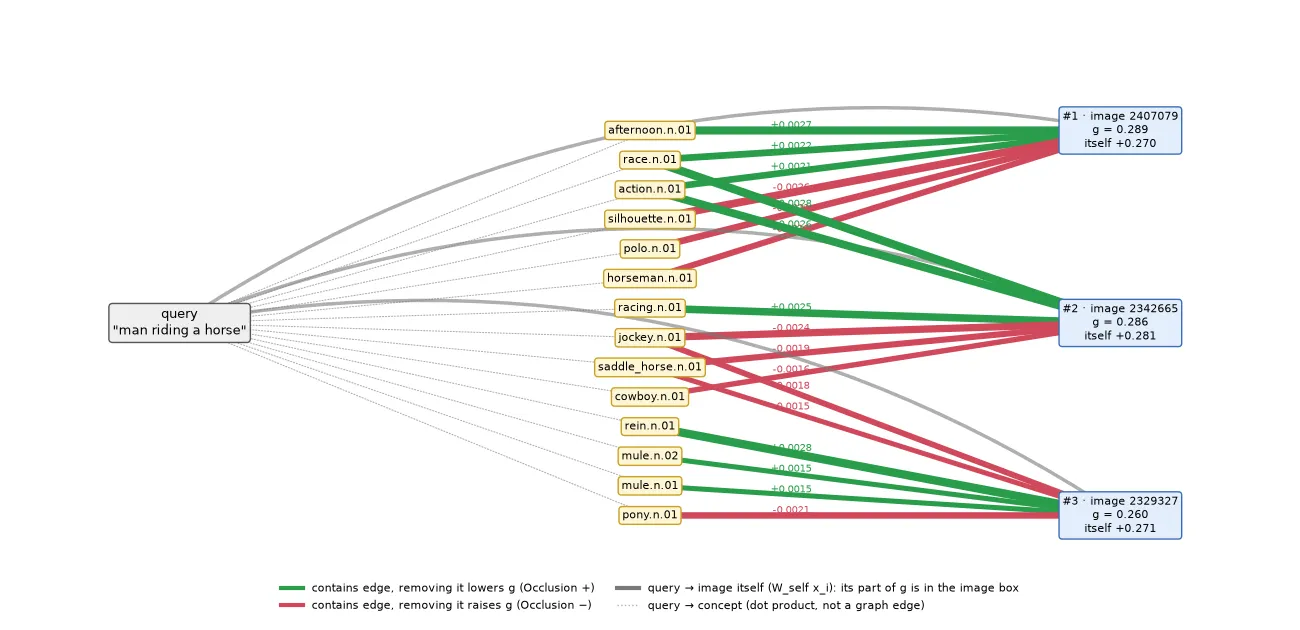
\includegraphics[width=0.8\textwidth]{query_path.png}
\caption{Giao diện demo cho truy vấn ``man riding a horse'': top-3 ảnh val và đường đi truy vấn $\to$ khái niệm $\to$ ảnh. Cạnh xanh là cạnh mà khi xóa thì điểm $g$ giảm; cạnh đỏ là cạnh kéo ảnh xuống. Ô ảnh ghi phần điểm đến từ chính ảnh ($W_{\text{self}}x_i$).}
\label{fig:demo}
\end{figure*}

\begin{figure}[t]
\centering
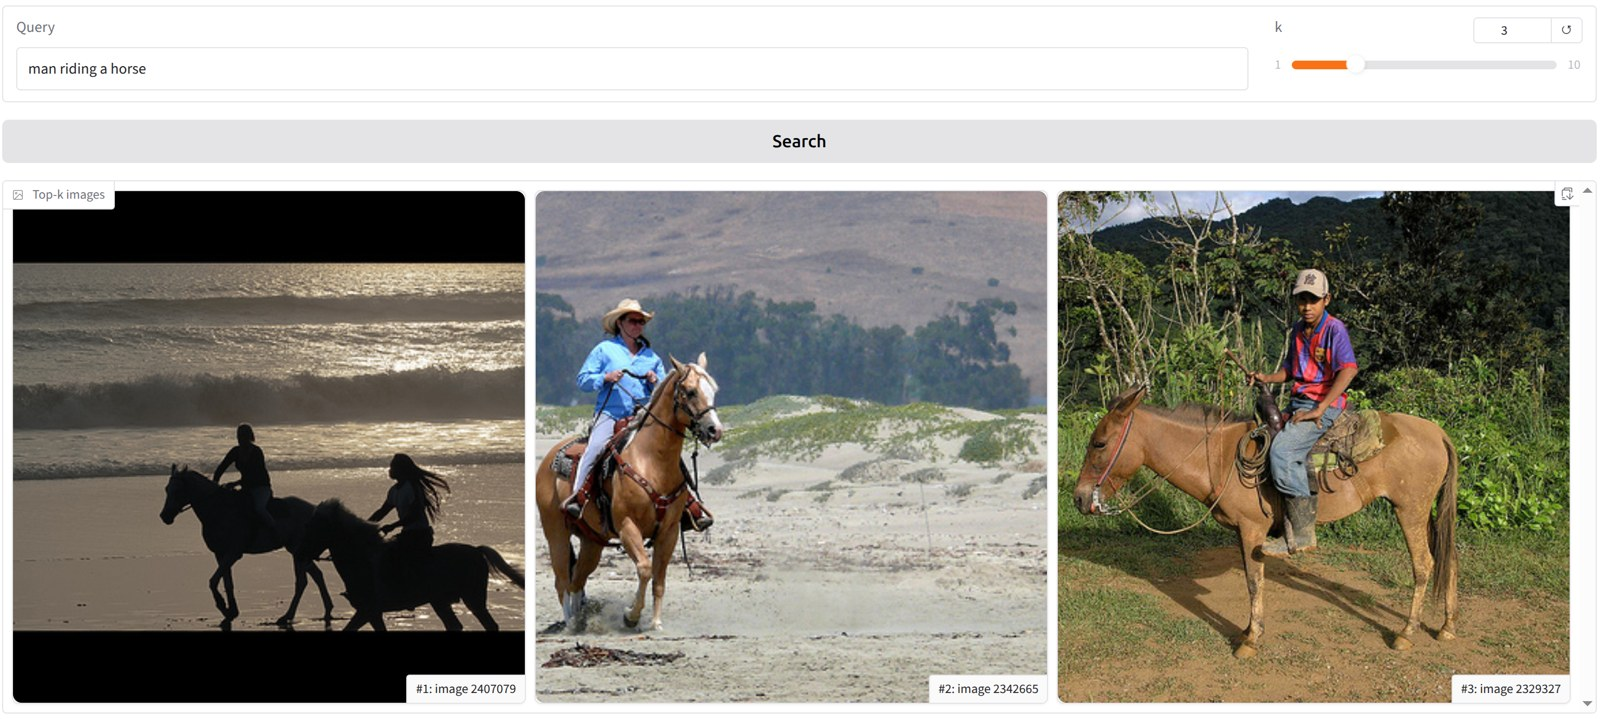
\includegraphics[width=\linewidth]{query_result.jpg}
\caption{Kết quả top-3 của demo cho truy vấn ``man riding a horse'' trên tập val Visual Genome.}
\label{fig:demo-result}
\end{figure}

Ứng dụng demo viết bằng Gradio (\code{app/gradio\_app.py}) nhận một câu truy vấn, trả về top-$k$ ảnh val (Hình~\ref{fig:demo-result}) và vẽ, cho từng ảnh, các cạnh \code{contains} đã tạo nên điểm đồ thị cùng đóng góp Occlusion có dấu của từng cạnh (Hình~\ref{fig:demo}). Giao diện chỉ gọi các hàm trong thư viện \code{src/mmxai/} của dự án, không chứa logic riêng, nên những gì hiển thị đúng là mô hình đã báo cáo. Ví dụ trong hình cho thấy cả những cạnh hợp nghĩa (\code{race}, \code{racing}, \code{rein}) lẫn những cạnh có đóng góp âm (\code{polo}, \code{jockey}). Demo chạy được trên máy không có GPU; hướng dẫn cài đặt nằm trong \code{app/README.md}.

\section{Thảo luận và hạn chế}
\label{sec:discussion}
\textit{Vai trò của đối chứng không đồ thị.} Nếu thiếu đối chứng này, toàn bộ mức tăng 19\% trên Visual Genome sẽ bị gán nhầm cho đồ thị. Kết luận ``phần lớn mức tăng đến từ phép chiếu học được'' lặp lại trên ba bộ dữ liệu (Visual Genome, Flickr30k, MMKG) và với cả G-Retriever. Đồ thị thật tốt hơn đồ thị xáo trên Visual Genome và Flickr30k, nhưng chỉ trên Visual Genome mô hình có đồ thị mới cao hơn mô hình không đồ thị; trên Flickr30k và MMKG thì không.

\textit{Thông tin trong đồ thị.} Cạnh \code{contains} được suy ra từ chính CLIP (16 khái niệm gần nhất), không có quan hệ giữa các đối tượng trong scene graph và chưa dùng ConceptNet. Lựa chọn này giúp hệ thống chạy được với ảnh chưa gán nhãn và tránh rò rỉ, nhưng khiến đồ thị mang ít thông tin mới so với những gì CLIP đã biết. Đây có lẽ là lý do chính khiến đồ thị chỉ giúp ở các truy vấn chung chung. Ngoài ra, cạnh ở mức cả ảnh không khớp với truy vấn mô tả một vùng nhỏ của Visual Genome.

\textit{Trọng số kết hợp.} Trên Visual Genome, $\alpha \approx 0$ khiến điểm cuối gần như chỉ còn nhánh học được, và các trường hợp thất bại lớn (hạng của ảnh đúng giảm từ 7--15 xuống 92--100) cho thấy một giá trị $\alpha$ chung cho mọi truy vấn là chưa phù hợp.

\textit{Giới hạn thống kê.} Mỗi thí nghiệm có 3 seed và chỉ có một bản xáo; t và $p$ tính theo seed chỉ mang tính mô tả. Nhóm chưa có kiểm định theo truy vấn. Recall là cận dưới vì mỗi ảnh chỉ xét 5 câu, MRR bị cắt ở 100, và hai câu khác chữ nhưng cùng nghĩa (``a man'', ``man'') vẫn được tính là khác nhau.

\textit{Giới hạn của MMKG.} Truy vấn được sinh bằng mẫu câu cố định, chưa có câu tự nhiên do người viết; mỗi nhóm chỉ có 35--80 câu; 2/158 câu gián tiếp vẫn để lộ tên hiện vật qua tên của thực thể đích. Nhóm chưa chạy ablation bỏ hoặc xáo bộ ba. Muốn chuyển ngôn ngữ thật sự, cần một bộ mã hóa văn bản đa ngôn ngữ; khi đó không gian vectơ thay đổi và phải huấn luyện lại GNN.

\textit{Phần chưa hoàn thành.} Bộ 38 truy vấn trực tiếp và gián tiếp trên test Visual Genome đã được xây, duyệt và chấm cho CLIP thuần, G-Retriever và đối chứng (Mục~\ref{sec:kgbench}); ba mô hình cấp độ 1 còn chờ checkpoint; cải tiến riêng của nhóm (cấp độ 4) chưa được thực hiện.

\section{Kết luận và hướng phát triển}
\label{sec:conclusion}
Đồ án xây dựng một hệ thống truy vấn ảnh bằng văn bản có đồ thị, với năm quy tắc chống rò rỉ (Mục~\ref{sec:data}) và giải thích được kiểm chứng bằng can thiệp. Trên Visual Genome, CLIP kết hợp GraphSAGE nâng \mrr{} test từ 0,1076 lên 0,1284. Các đối chứng cho thấy khoảng 91\% mức tăng đến từ phép chiếu học được; cấu trúc ảnh--khái niệm thật đóng góp phần nhỏ nhưng ổn định so với đồ thị xáo, rõ nhất ở các truy vấn chung chung. Việc phần lớn mức tăng đến từ phép chiếu lặp lại trên Flickr30k, trên MMKG tiếng Việt và với phần truy xuất đồ thị con của G-Retriever; ở ba thí nghiệm này, đồ thị không tốt hơn mô hình không đồ thị. Giải thích bằng Integrated Gradients trung thực với mô hình trên cả Visual Genome lẫn MMKG, với mức tụt hạng khi bỏ cạnh giải thích lớn hơn nhiều so với bỏ cạnh ngẫu nhiên.

Nhóm đề xuất ba hướng tiếp theo. Thứ nhất, học $\alpha(q)$ thay đổi theo từng truy vấn thay cho một $\alpha$ cố định, nhắm vào các trường hợp thất bại ở Bảng~\ref{tab:case}. Thứ hai, thêm cạnh quan hệ từ scene graph và ConceptNet để kiểm chứng giả thuyết rằng đồ thị giàu quan hệ giúp ích cho truy vấn gián tiếp. Thứ ba, dùng bộ mã hóa văn bản đa ngôn ngữ để truy vấn tiếng Việt có thể khai thác được MMKG.

\section*{Khai báo sử dụng AI}
Nhóm dùng Claude Code để hỗ trợ viết mã, kiểm thử, tài liệu ADR, rà soát mã và soạn bản nháp báo cáo. Mọi lần sử dụng được ghi trong \code{docs/ai-usage-log.md} của kho mã. Số liệu trong báo cáo được chép từ \code{results/tables/}, không tính lại. Các thành viên đã đọc lại toàn bộ nội dung và chịu trách nhiệm giải thích mọi phần khi vấn đáp.

\begin{thebibliography}{00}
\bibitem{radford2021clip} A. Radford \textit{et al.}, ``Learning transferable visual models from natural language supervision,'' in \textit{Proc. ICML}, 2021.
\bibitem{cherti2023openclip} M. Cherti \textit{et al.}, ``Reproducible scaling laws for contrastive language-image learning,'' in \textit{Proc. CVPR}, 2023.
\bibitem{schuhmann2022laion} C. Schuhmann \textit{et al.}, ``LAION-5B: An open large-scale dataset for training next generation image-text models,'' in \textit{NeurIPS Datasets and Benchmarks}, 2022.
\bibitem{johnson2019faiss} J. Johnson, M. Douze, and H. Jégou, ``Billion-scale similarity search with GPUs,'' \textit{IEEE Trans. Big Data}, 2019.
\bibitem{krishna2017vg} R. Krishna \textit{et al.}, ``Visual Genome: Connecting language and vision using crowdsourced dense image annotations,'' \textit{Int. J. Comput. Vis.}, 2017.
\bibitem{young2014flickr} P. Young, A. Lai, M. Hodosh, and J. Hockenmaier, ``From image descriptions to visual denotations,'' \textit{Trans. Assoc. Comput. Linguist.}, 2014.
\bibitem{karpathy2015} A. Karpathy and L. Fei-Fei, ``Deep visual-semantic alignments for generating image descriptions,'' in \textit{Proc. CVPR}, 2015.
\bibitem{miller1995wordnet} G. A. Miller, ``WordNet: A lexical database for English,'' \textit{Commun. ACM}, 1995.
\bibitem{speer2017conceptnet} R. Speer, J. Chin, and C. Havasi, ``ConceptNet 5.5: An open multilingual graph of general knowledge,'' in \textit{Proc. AAAI}, 2017.
\bibitem{kipf2017gcn} T. N. Kipf and M. Welling, ``Semi-supervised classification with graph convolutional networks,'' in \textit{Proc. ICLR}, 2017.
\bibitem{velickovic2018gat} P. Veličković \textit{et al.}, ``Graph attention networks,'' in \textit{Proc. ICLR}, 2018.
\bibitem{hamilton2017sage} W. Hamilton, Z. Ying, and J. Leskovec, ``Inductive representation learning on large graphs,'' in \textit{Proc. NeurIPS}, 2017.
\bibitem{fey2019pyg} M. Fey and J. E. Lenssen, ``Fast graph representation learning with PyTorch Geometric,'' in \textit{ICLR Workshop on Representation Learning on Graphs and Manifolds}, 2019.
\bibitem{oord2018cpc} A. van den Oord, Y. Li, and O. Vinyals, ``Representation learning with contrastive predictive coding,'' arXiv:1807.03748, 2018.
\bibitem{church1990pmi} K. Church and P. Hanks, ``Word association norms, mutual information, and lexicography,'' \textit{Comput. Linguist.}, 1990.
\bibitem{jarvelin2002ndcg} K. Järvelin and J. Kekäläinen, ``Cumulated gain-based evaluation of IR techniques,'' \textit{ACM Trans. Inf. Syst.}, 2002.
\bibitem{chen2024kgmm} Z. Chen \textit{et al.}, ``Knowledge graphs meet multi-modal learning: A comprehensive survey,'' arXiv:2402.05391, 2024.
\bibitem{chen2022mkgformer} X. Chen \textit{et al.}, ``Hybrid transformer with multi-level fusion for multimodal knowledge graph completion,'' in \textit{Proc. SIGIR}, 2022.
\bibitem{zhang2024native} Y. Zhang \textit{et al.}, ``NativE: Multi-modal knowledge graph completion in the wild,'' in \textit{Proc. SIGIR}, 2024.
\bibitem{zhang2024adamf} Y. Zhang \textit{et al.}, ``Unleashing the power of imbalanced modality information for multi-modal knowledge graph completion,'' in \textit{Proc. LREC-COLING}, 2024.
\bibitem{he2024gretriever} X. He \textit{et al.}, ``G-Retriever: Retrieval-augmented generation for textual graph understanding and question answering,'' in \textit{Proc. NeurIPS}, 2024.
\bibitem{hegde2015pcst} C. Hegde, P. Indyk, and L. Schmidt, ``A nearly-linear time framework for graph-structured sparsity,'' in \textit{Proc. ICML}, 2015.
\bibitem{sundararajan2017ig} M. Sundararajan, A. Taly, and Q. Yan, ``Axiomatic attribution for deep networks,'' in \textit{Proc. ICML}, 2017.
\bibitem{ying2019gnnexplainer} Z. Ying \textit{et al.}, ``GNNExplainer: Generating explanations for graph neural networks,'' in \textit{Proc. NeurIPS}, 2019.
\bibitem{amara2022graphframex} K. Amara \textit{et al.}, ``GraphFramEx: Towards systematic evaluation of explainability methods for graph neural networks,'' in \textit{Proc. LoG}, 2022.
\bibitem{zheng2024robust} X. Zheng \textit{et al.}, ``Towards robust fidelity for evaluating explainability of GNNs,'' in \textit{Proc. ICLR}, 2024.
\bibitem{wilcoxon1945} F. Wilcoxon, ``Individual comparisons by ranking methods,'' \textit{Biometrics Bulletin}, 1945.
\end{thebibliography}

%======================================================================
% Phụ lục: đặt sau Tài liệu tham khảo, không tính vào giới hạn số trang
\appendices

\section{Bảng phân công công việc}
\label{app:tasks}
\begin{table}[h]
\centering
\caption{Phân công công việc và tỉ lệ đóng góp của từng thành viên}
\label{tab:tasks}
\scriptsize
\setlength{\tabcolsep}{2pt}
\begin{tabular}{@{}c p{1.1cm} p{1.3cm} p{3.9cm} c@{}}
\toprule
\textbf{STT} & \textbf{MSHV} & \textbf{Họ và tên} & \textbf{Công việc} & \textbf{Tỉ lệ} \\
\midrule
1 & … & … & … & … \\
2 & … & … & … & … \\
3 & 25C15060 & Nguyễn Phước Thiện & Viết các hàm dùng chung cho giải thích cơ bản và giải thích định lượng; dựng demo hiển thị kết quả và đường đi; chạy thực nghiệm trên Flickr30k; viết báo cáo cho các phần trên & … \\
4 & 25C15050 & Quan Phú Long & Trích đặc trưng CLIP (Flickr30k, Visual Genome) và notebook Kaggle; dựng đồ thị ảnh--khái niệm; GraphSAGE, xếp hạng lại, chọn $\alpha$, cạnh đồng xuất hiện; duyệt MMKG; đánh giá chuyển giao và đánh giá giải thích trên MMKG; viết phần MMKG và tài liệu hướng dẫn & … \\
5 & 25C15068 & Trần Hồ Thanh Vũ & Theo dõi tiến độ; viết báo cáo; làm slide; hỗ trợ nhóm & … \\
\bottomrule
\end{tabular}
\end{table}


\end{document}
